% ============================================================================
% UBT Scintillator Digitization -- Beamer slide deck
% Companion presentation to documentation/main.tex
% Compile with pdflatex (run twice for the table of contents / references).
% ============================================================================
\documentclass[aspectratio=169,10pt]{beamer}

\usepackage[utf8]{inputenc}
\usepackage[T1]{fontenc}
\usepackage{lmodern}
\usepackage{textcomp}
\usepackage{amsmath,amssymb}
\usepackage{booktabs}
\usepackage{graphicx}
\usepackage{tikz}
\usetikzlibrary{arrows.meta,positioning}

\usetheme{Boadilla}
\usecolortheme{seahorse}
\setbeamertemplate{navigation symbols}{}
\setbeamertemplate{caption}[numbered]
\setbeamertemplate{footline}[frame number]
\setbeamercovered{transparent}
% NOTE: enumitem is deliberately NOT used. Loading it together with
% beamer's own \enumerate implementation causes infinite macro
% recursion in \labelenumi ("TeX capacity exceeded") the moment any
% \begin{enumerate} appears, regardless of \setlist scoping. Itemize
% spacing is instead tightened per-list with \itemsep/\parskip below.
\renewcommand{\arraystretch}{0.9}

% ---------------------------------------------------------------------------
% Title data
% ---------------------------------------------------------------------------
\title[UBT Digitization]{UBT Scintillator Digitization}
\subtitle{Geometry, Optical Model, and ADC Digitizer Validation for the
  SHiP Upstream Background Tagger}
\author{V.~Kholoimov}
\institute[EPFL]{EPFL \\ \textit{SHiP Experiment, CERN}}
\date{\today}

% Convenience macros matching documentation/implementation.tex notation
\newcommand{\muminus}{\ensuremath{\mu^{-}}}
\newcommand{\eminus}{\ensuremath{e^{-}}}
\newcommand{\gam}{\ensuremath{\gamma}}

% Note: no shared \graphicspath is used, since several figures share the
% same basename across plots/, plots_20mm/, and adc/ subfolders. Every
% \includegraphics call below therefore gives its full relative path.

\begin{document}

% ---------------------------------------------------------------------------
\begin{frame}
  \titlepage
\end{frame}

\begin{frame}{Outline}
  \tableofcontents
\end{frame}

% ============================================================================
\section{Detector Definition}
% ============================================================================

\begin{frame}{Geometry \& Sensor Stack}
  \begin{columns}[T]
    \begin{column}{0.52\textwidth}
      \footnotesize
      \textbf{Volumes}
      \begin{itemize}
        \item World: Geant4 air box, half-size $(0.5,0.5,0.5)~\mathrm{m}$.
        \item Default tile: $40\times40\times10~\mathrm{mm^3}$.
        \item \texttt{UBT\_SCINTILLATOR\_SIZE\_MM=20} selects
          $20\times20\times5~\mathrm{mm^3}$; other sizes rejected.
        \item Sensor active face fixed at $6\times6~\mathrm{mm^2}$ for
          both tile sizes.
      \end{itemize}
      \vspace{3pt}
      \textbf{Coordinate convention}
      \begin{itemize}
        \item Scintillator center at $(0,0,0)$; beam along $+z$; sensor
          stack on the $+z$ face.
        \item Muon source plane upstream at negative $z$.
        \item Gun default: \muminus\ at $(0,0,-30~\mathrm{mm})$, direction
          $(0,0,1)$; kinetic energy uniform in $1$--$20~\mathrm{GeV}$.
      \end{itemize}
    \end{column}
    \begin{column}{0.48\textwidth}
      \centering
      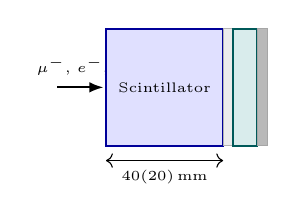
\begin{tikzpicture}[scale=0.62, every node/.style={font=\tiny}]
        \draw[-{Latex[length=1.8mm]}, thick] (-1.0,1.2) -- (-0.05,1.2);
        \node[anchor=south] at (-0.5,1.25) {\muminus, \eminus, \gam};
        \draw[fill=blue!12, draw=blue!60!black, thick] (0,0) rectangle (2.4,2.4);
        \node at (1.2,1.2) {Scintillator};
        \draw[fill=gray!15, draw=gray!60] (2.4,0) rectangle (2.6,2.4);
        \draw[fill=teal!15, draw=teal!70!black, thick] (2.6,0) rectangle (3.1,2.4);
        \draw[fill=gray!55, draw=gray!70] (3.1,0) rectangle (3.3,2.4);
        \draw[<->] (0,-0.3) -- (2.4,-0.3) node[midway, below] {40(20)\,mm};
      \end{tikzpicture}

      \vspace{2pt}
      {\scriptsize\raggedright
      $p$-terphenyl+POPOP scintillator $\to$ grease (0.2\,mm) $\to$ glass
      window (1.0\,mm) $\to$ photocathode/SiPM (0.1\,mm).\par}

      \vspace{4pt}
      \scriptsize
      \begin{tabular}{lcc}
        \toprule
        Parameter & 40\,mm tile & 20\,mm tile \\
        \midrule
        Transverse size & $40\times40$ & $20\times20$ \\
        Thickness & 10\,mm & 5\,mm \\
        Sensor face & \multicolumn{2}{c}{$6\times6~\mathrm{mm^2}$} \\
        Beam-spot half-size $a$ & 20\,mm (init.) & $\le 10$\,mm \\
        \bottomrule
      \end{tabular}
    \end{column}
  \end{columns}
\end{frame}

\begin{frame}{Materials, Optics \& Timing Model}
  \begin{columns}[T]
    \begin{column}{0.52\textwidth}
      \footnotesize
      \textbf{Materials}
      \begin{itemize}
        \item Scintillator: effective para-terphenyl + POPOP,
          $\rho = 1.23~\mathrm{g/cm^3}$; bulk composition
          $\mathrm{C_{18}H_{14}}$. POPOP enters via the emission
          spectrum, not as an explicit dopant fraction.
        \item Window: Pyrex glass \quad Grease: hydrocarbon \quad
          Photocathode: silicon slab \quad World: air.
      \end{itemize}
      \vspace{3pt}
      \textbf{Photon detection chain}
      \begin{itemize}
        \item Two Bernoulli filters at the photocathode boundary: flat
          light-collection $\epsilon_\mathrm{LC}=0.30$, then
          energy-dependent $\epsilon_\mathrm{PDE}(E_\gamma)$.
        \item Reference: Hamamatsu S13360-6050PE
          ($6\times6~\mathrm{mm^2}$, 50\,\textmu m pitch);
          $\epsilon_\mathrm{PDE}(450~\mathrm{nm})=40\%$.
        \item Digitizer gain $G=2.8\times10^6$;
          $\mathrm{ADC}=\mathrm{round}(Q[\mathrm{pC}])$ -- one pC equals
          one ADC count.
      \end{itemize}
    \end{column}
    \begin{column}{0.48\textwidth}
      \scriptsize
      \begin{tabular}{lc}
        \toprule
        \multicolumn{2}{l}{\textbf{Timing constants}} \\
        \midrule
        $\tau_\mathrm{rise}$ & 0.7\,ns \\
        $\tau_\mathrm{fast}$ & 2.0348\,ns \\
        $\tau_\mathrm{slow}$ & 11.3607\,ns \\
        $Y_\mathrm{fast}$ & 0.889145 \\
        $Y_\mathrm{slow}$ & 0.110855 \\
        Total yield & 10\,000\,$\gamma$/MeV \\
        \bottomrule
      \end{tabular}

      \vspace{6pt}
      \raggedright
      Shared emission spectrum (fast \emph{and} slow components) peaks at
      2.93\,eV (relative intensity 1.00), spanning
      2.75--3.10\,eV -- the two components differ only in time structure
      and relative yield, not spectral shape.
    \end{column}
  \end{columns}
\end{frame}

% ============================================================================
\section{Simulation \& Digitizer Results}
% ============================================================================

\begin{frame}{Scintillation Timing Model Validation}
  \begin{columns}[T]
    \begin{column}{0.6\textwidth}
      \centering
      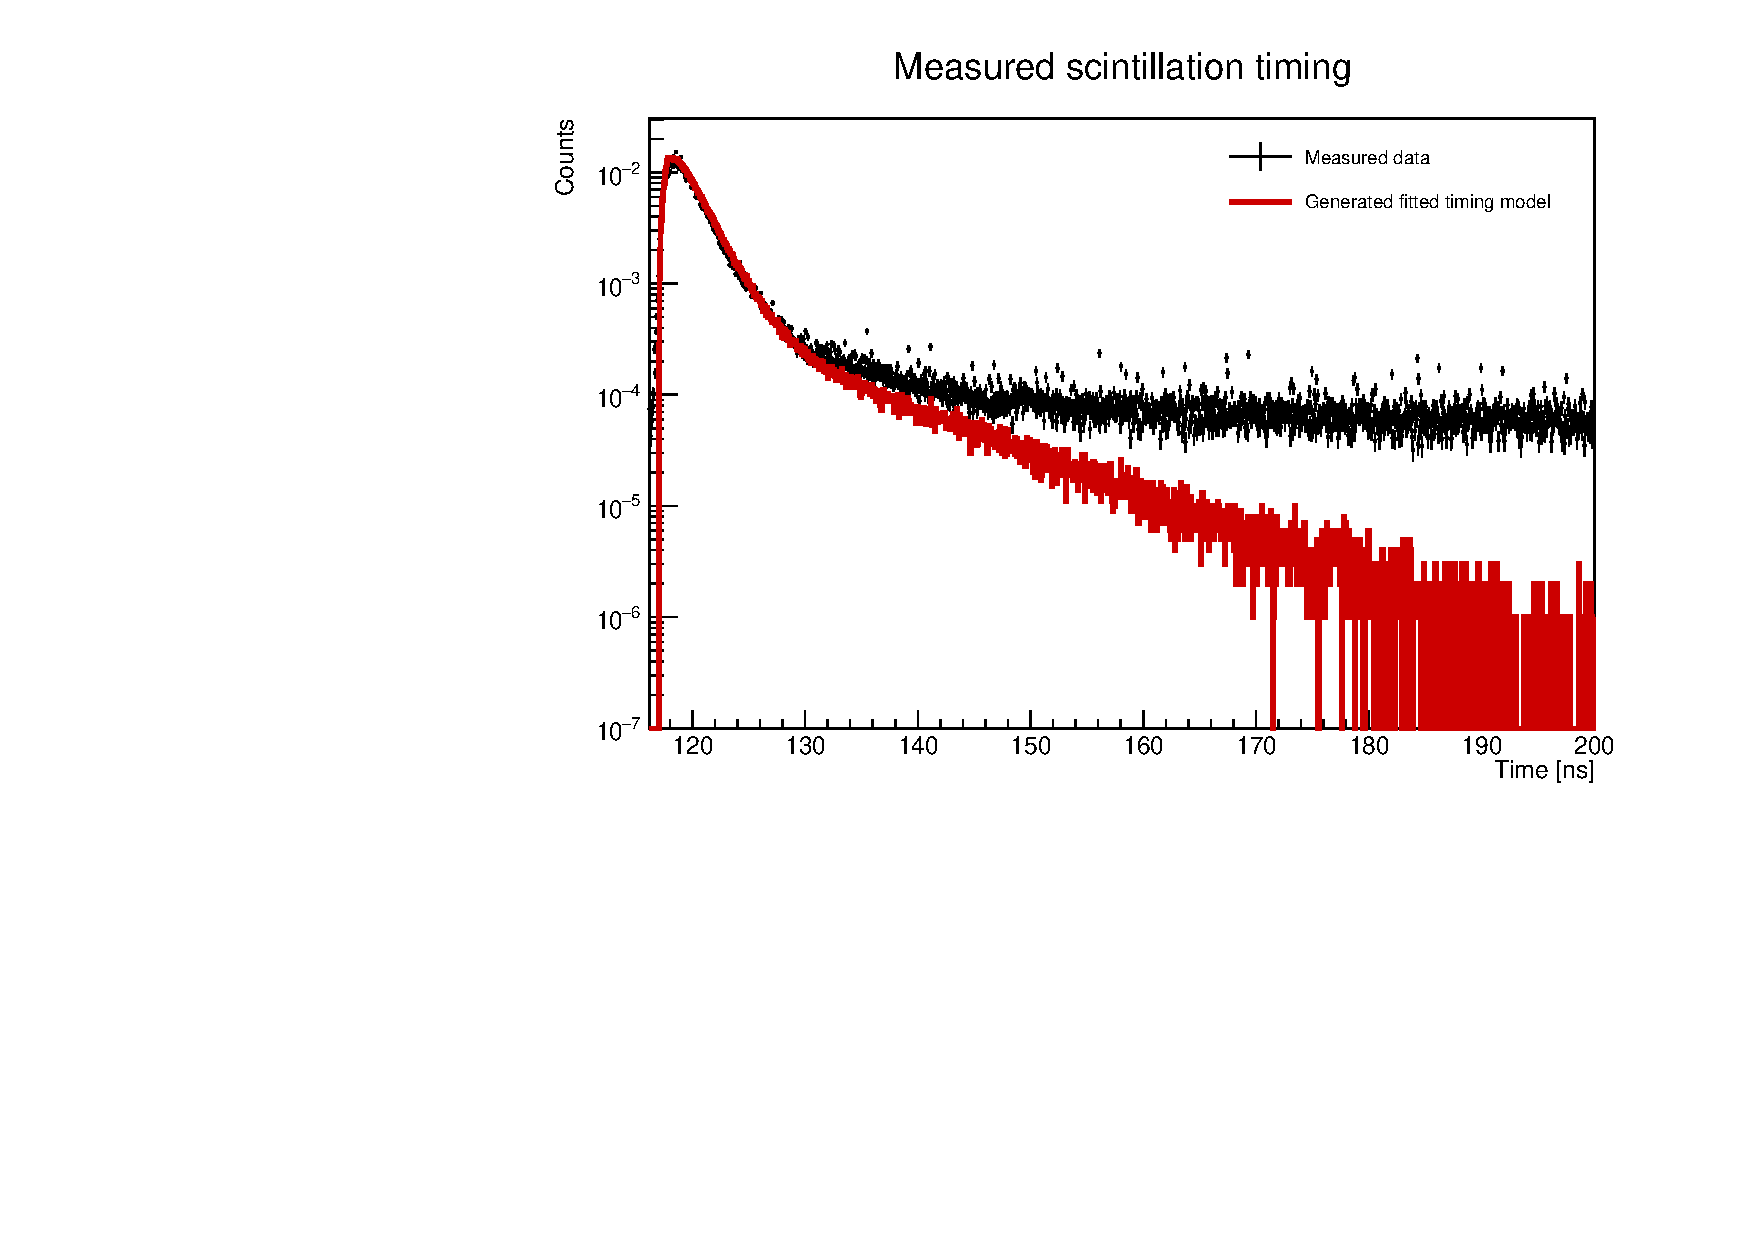
\includegraphics[height=3.2cm]{../analysis/scintillation_real_vs_generated.pdf}\\[2pt]
      \footnotesize Normalized measured spectrum compared with times
      generated from the fitted two-component model.
    \end{column}
    \begin{column}{0.4\textwidth}
      \centering
      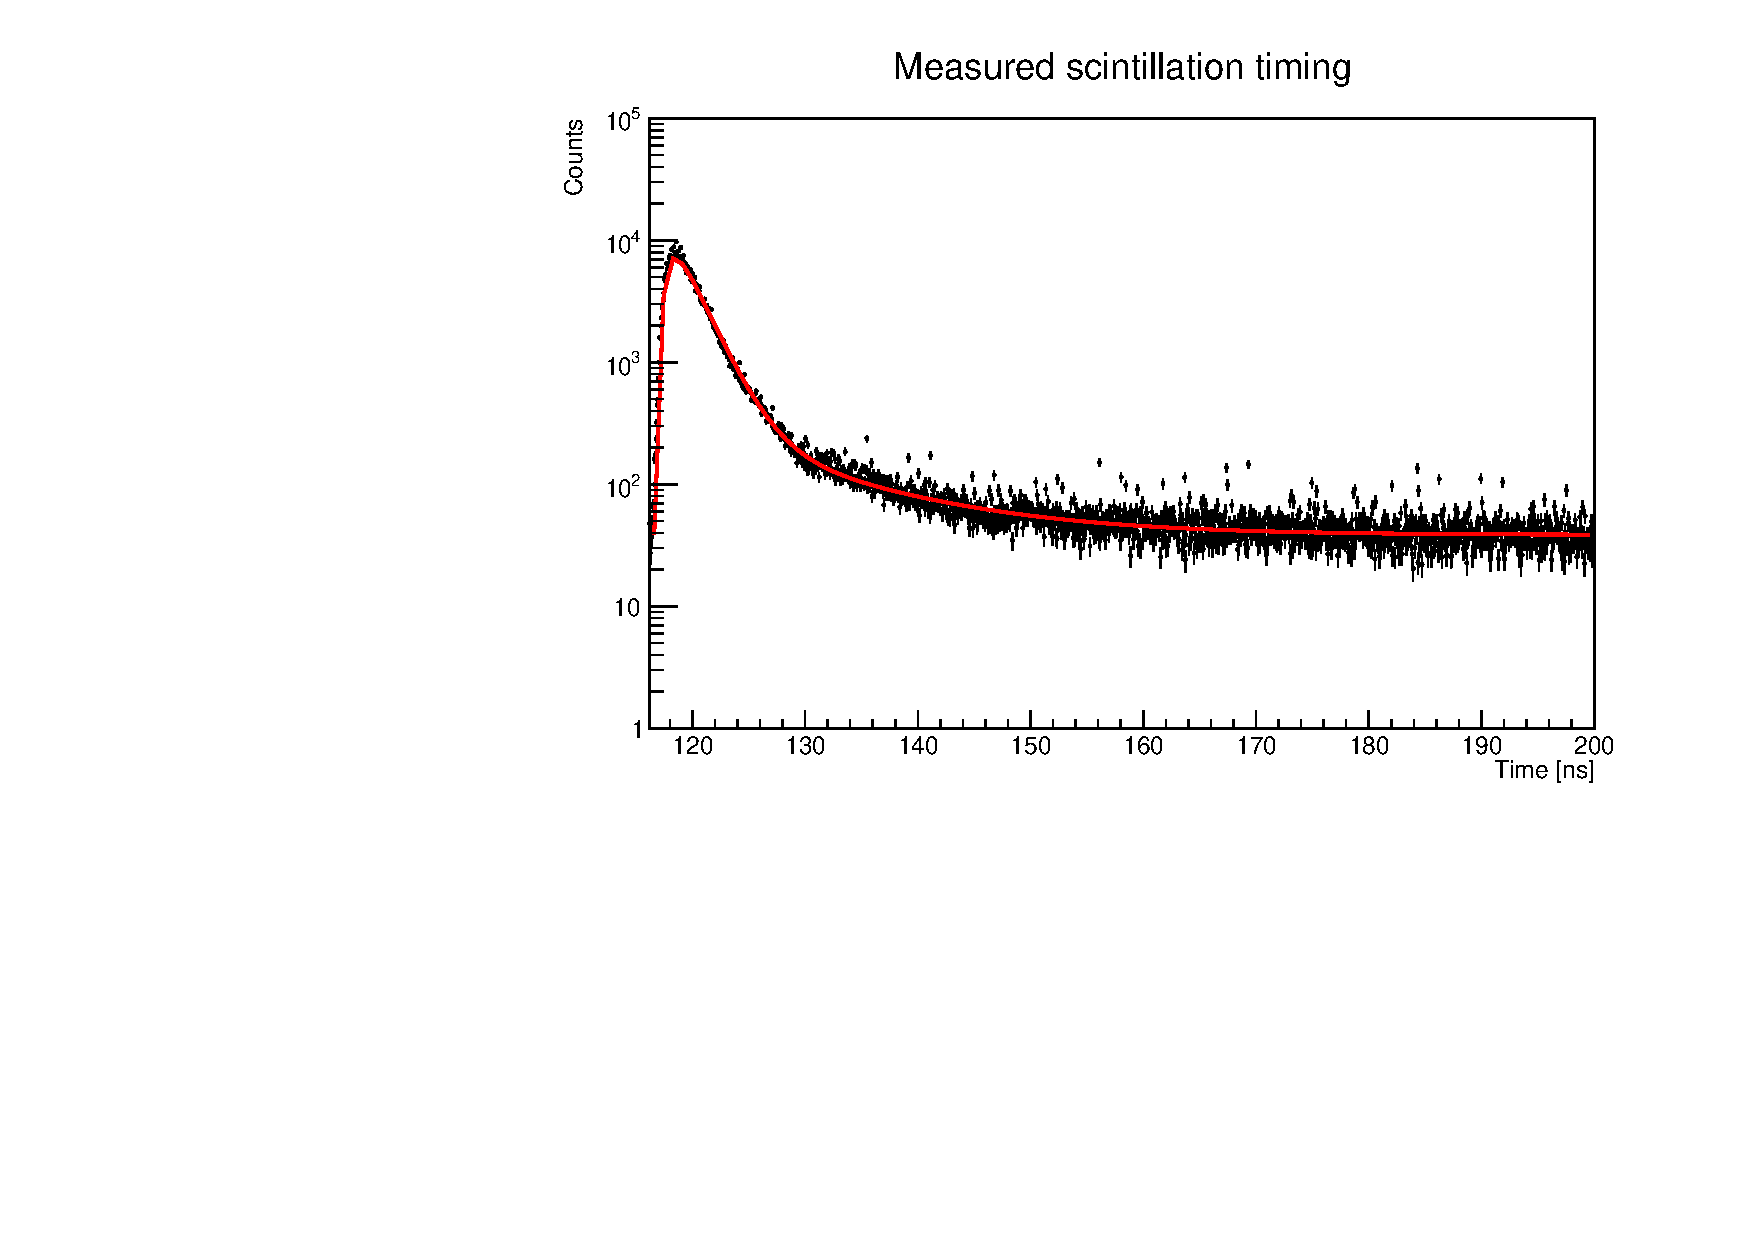
\includegraphics[height=2.6cm]{../analysis/scintillation_real_data.pdf}\\[2pt]
      \tiny Input: measured spectrum over the fit interval.

      \vspace{4pt}
      \raggedright\footnotesize
      One million times are generated from the fitted common-rise,
      fast-decay, slow-decay components (fixed seed). Both histograms are
      normalized, so the overlay tests timing \emph{shape} only.
    \end{column}
  \end{columns}
\end{frame}

\begin{frame}{Simulated Integrated PMT-Charge Distributions}
  \begin{columns}[T]
    \begin{column}{0.5\textwidth}
      \centering
      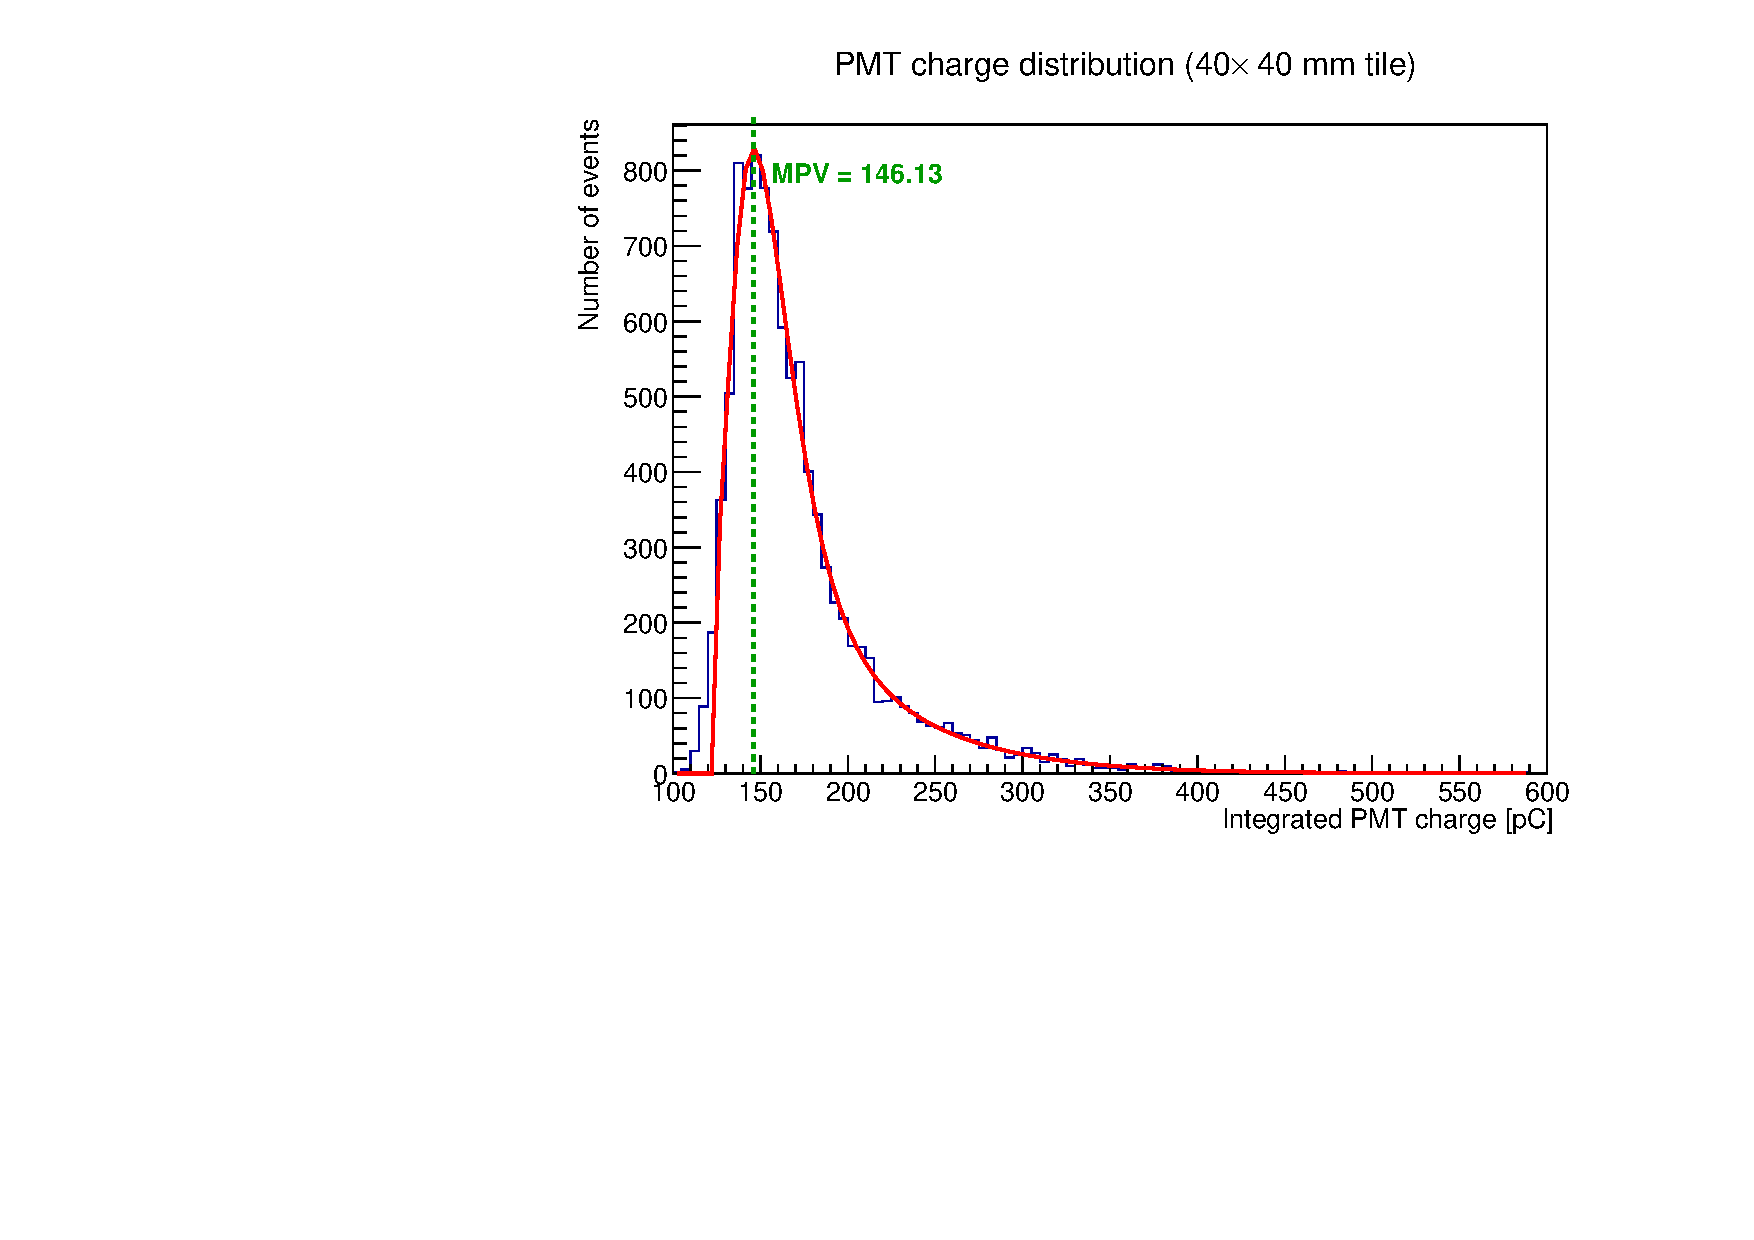
\includegraphics[height=3.0cm]{../analysis/plots/photoelectrons.pdf}\\[2pt]
      \footnotesize $40\times40~\mathrm{mm^2}$ tile
    \end{column}
    \begin{column}{0.5\textwidth}
      \centering
      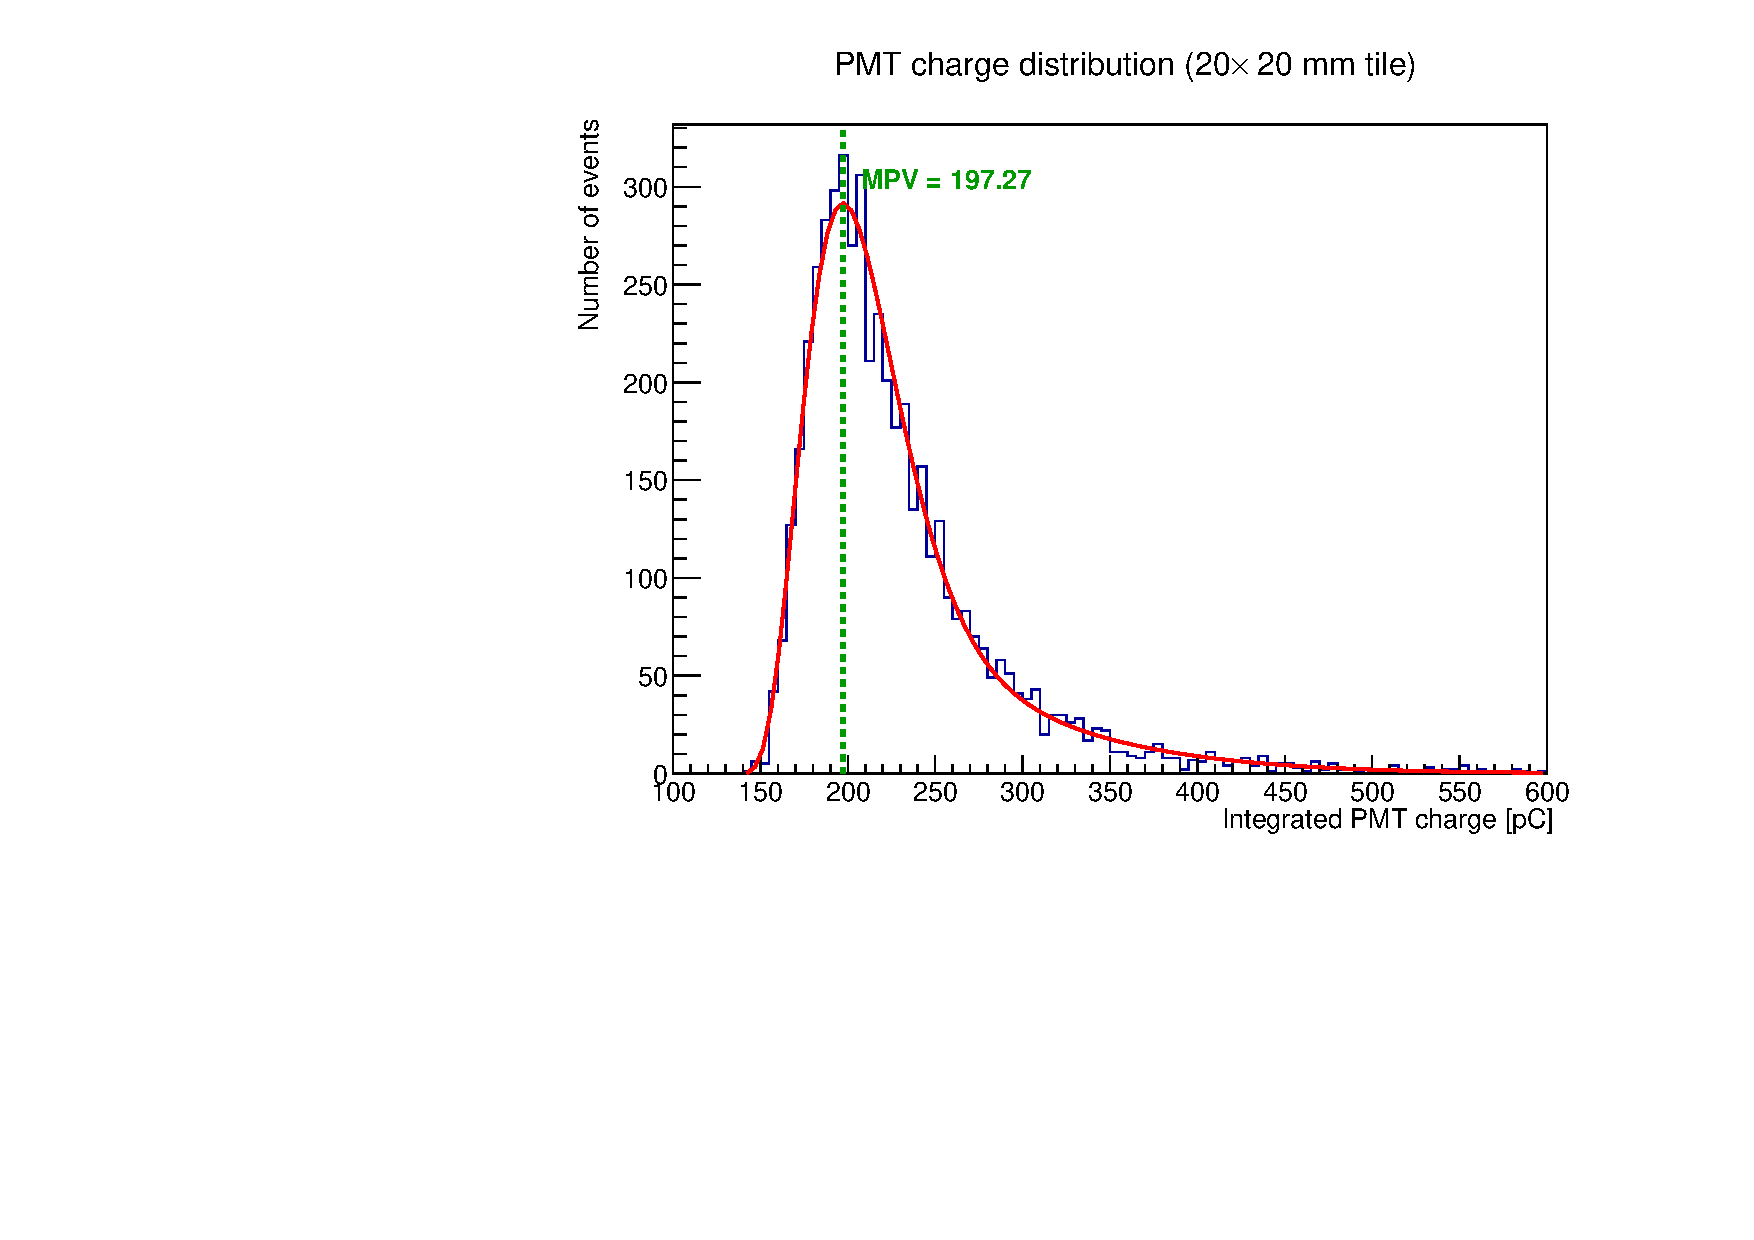
\includegraphics[height=3.0cm]{../analysis/plots_20mm/photoelectrons.pdf}\\[2pt]
      \footnotesize $20\times20~\mathrm{mm^2}$ tile
    \end{column}
  \end{columns}
  \vspace{4pt}
  \footnotesize
  Simulated integrated PMT-charge distributions in picocoulombs for the
  two tile sizes. Numerically, one pC corresponds to one ADC count in the
  present standalone conversion, but the plotted observable and
  horizontal axis are PMT charge in pC.
\end{frame}

\begin{frame}{Absolute Photoelectron-Arrival Timing}
  \begin{columns}[T]
    \begin{column}{0.5\textwidth}
      \centering
      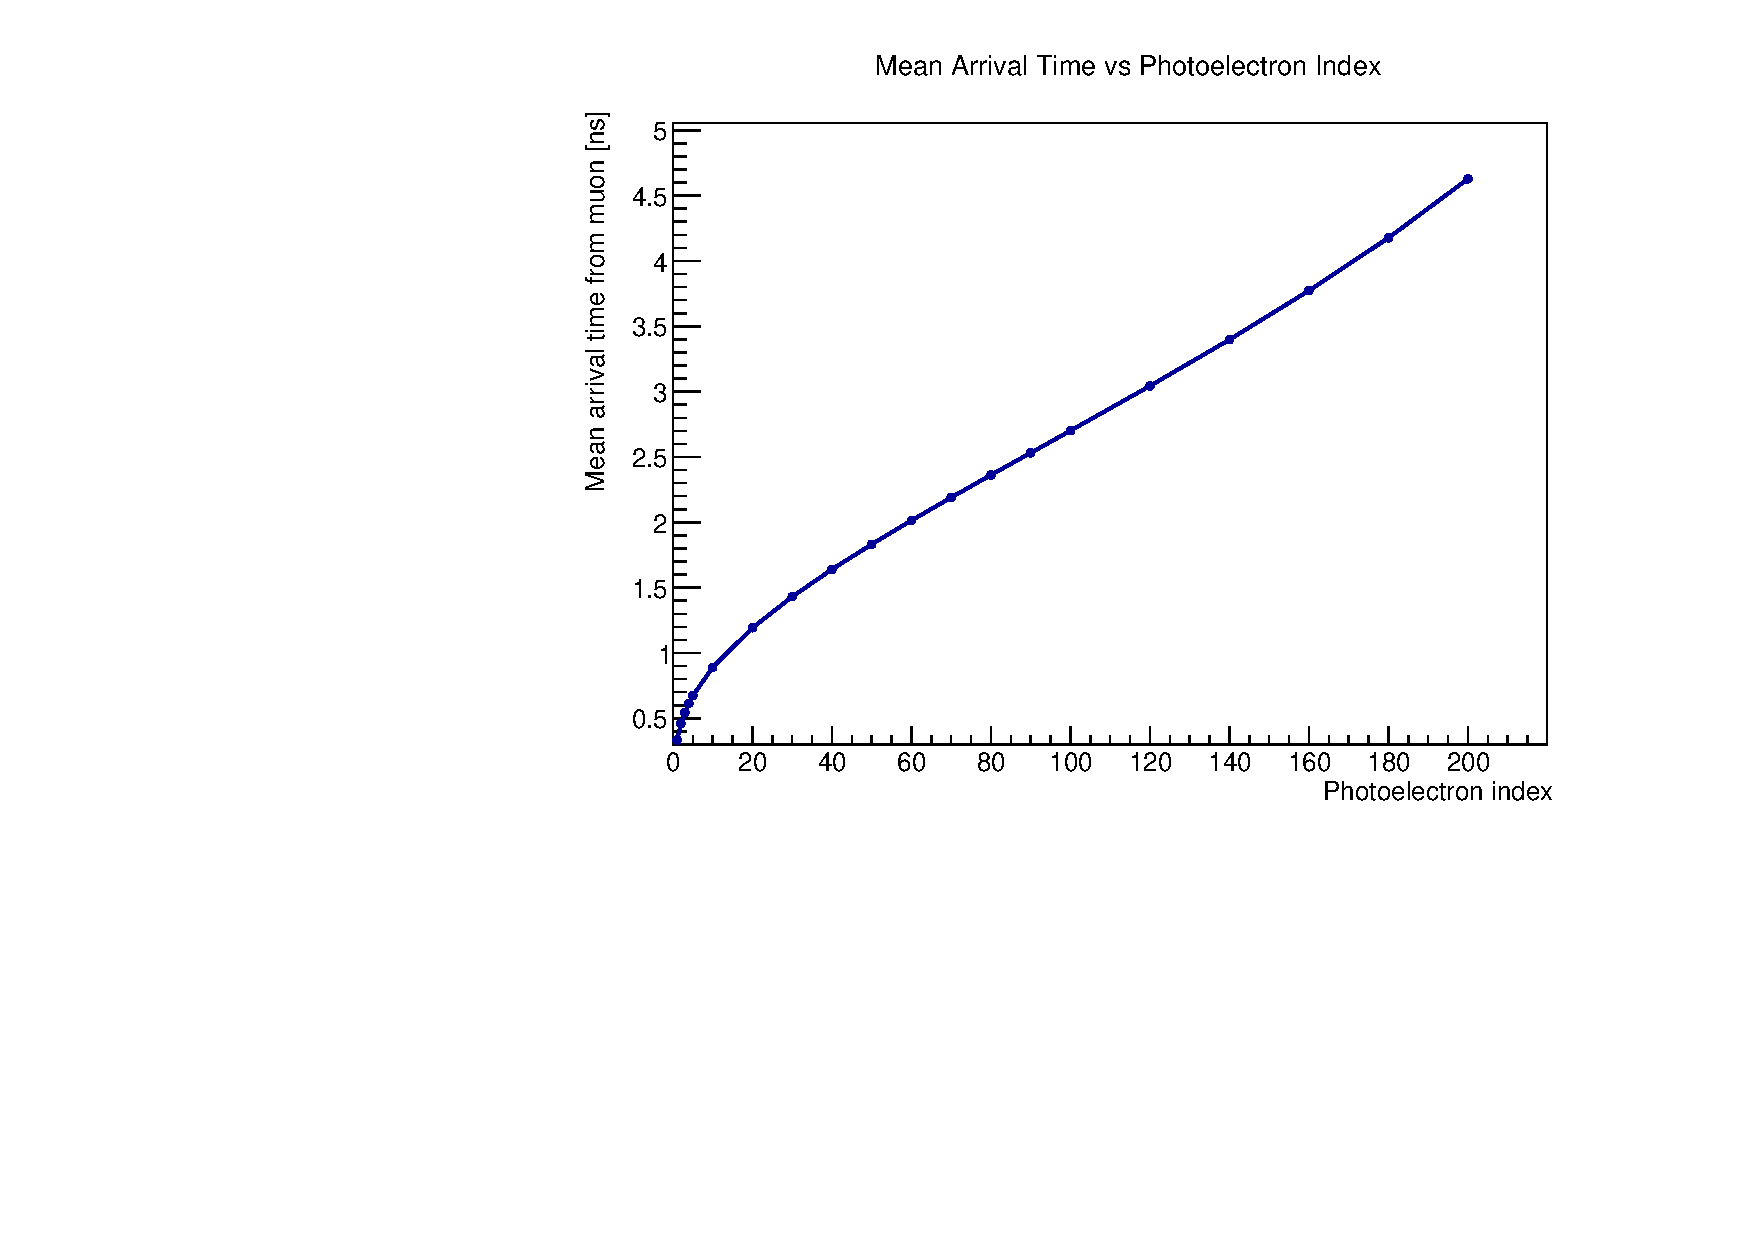
\includegraphics[height=2.5cm]{../analysis/plots/mean_arrival_time_vs_pe_index.pdf}\\[2pt]
      \footnotesize Mean arrival time $t_N$
    \end{column}
    \begin{column}{0.5\textwidth}
      \centering
      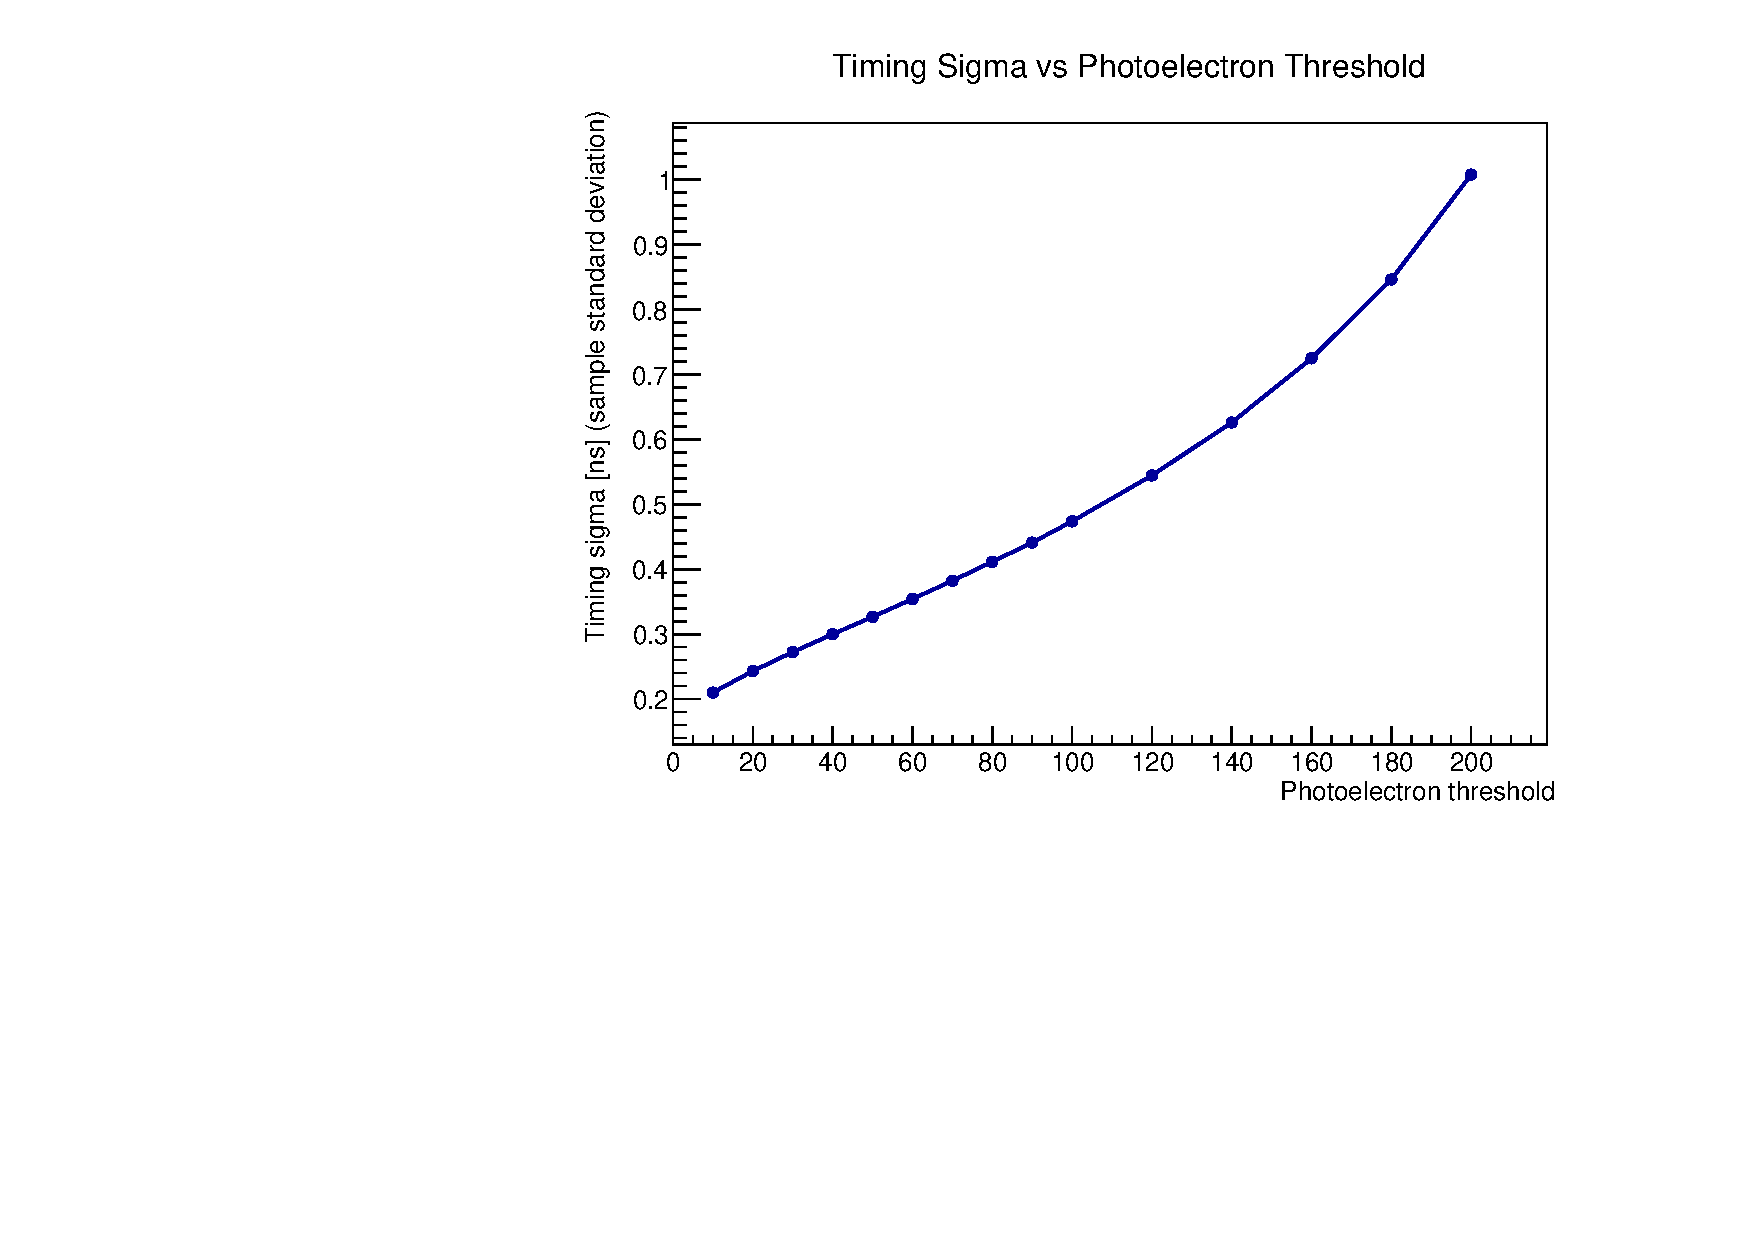
\includegraphics[height=2.5cm]{../analysis/plots/timing_sigma_vs_threshold.pdf}\\[2pt]
      \footnotesize Resolution $\sigma_{t_N}$
    \end{column}
  \end{columns}
  \vspace{3pt}
  \footnotesize
  Mean and resolution of the photoelectron-arrival time $t_N$ vs.\
  threshold $N$, from per-event values (no binning or fit); plotted only
  where $N$ has $\ge 10$ contributing events.

  \vspace{3pt}
  \begin{alertblock}{\footnotesize Preliminary timing study}
    \footnotesize Simulated timing does not yet agree with real tile
    measurements; FairShip uses a real-data-based timing smearing
    instead of this standalone response.
  \end{alertblock}
\end{frame}

\begin{frame}{Spatial Uniformity of the ADC Response}
  \begin{columns}[T]
    \begin{column}{0.5\textwidth}
      \centering
      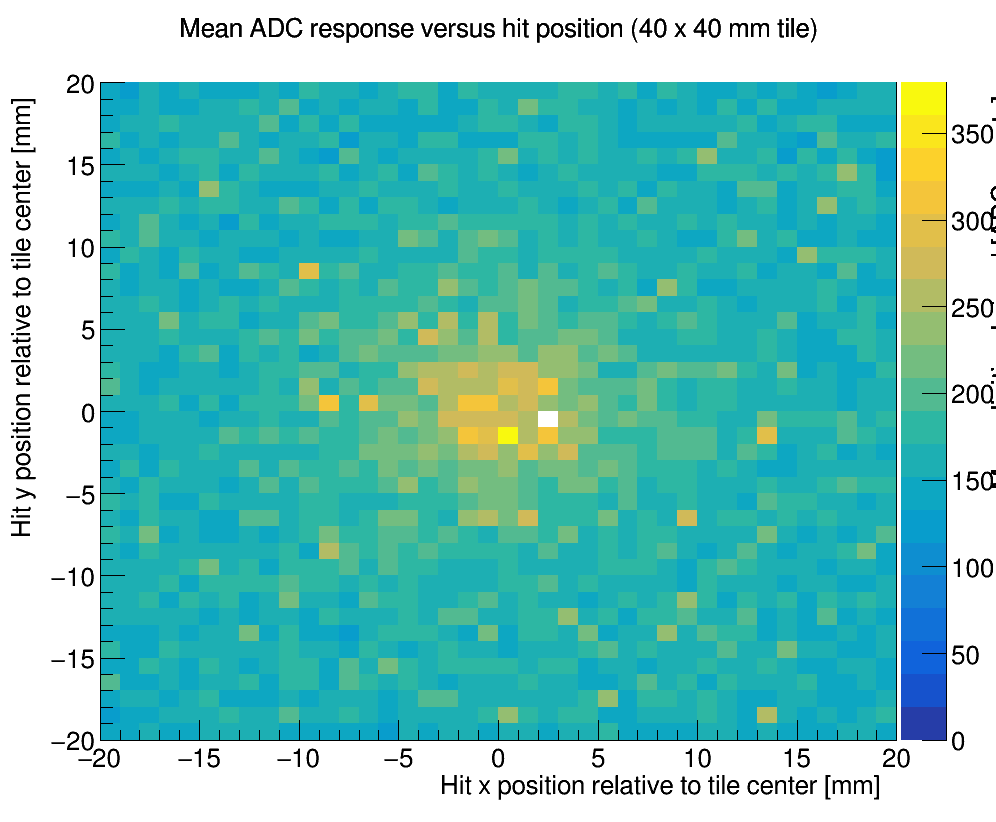
\includegraphics[height=3.0cm]{../analysis/plots/adc/mean_adc_vs_position.png}\\[2pt]
      \footnotesize Raw mean ADC vs.\ position
    \end{column}
    \begin{column}{0.5\textwidth}
      \centering
      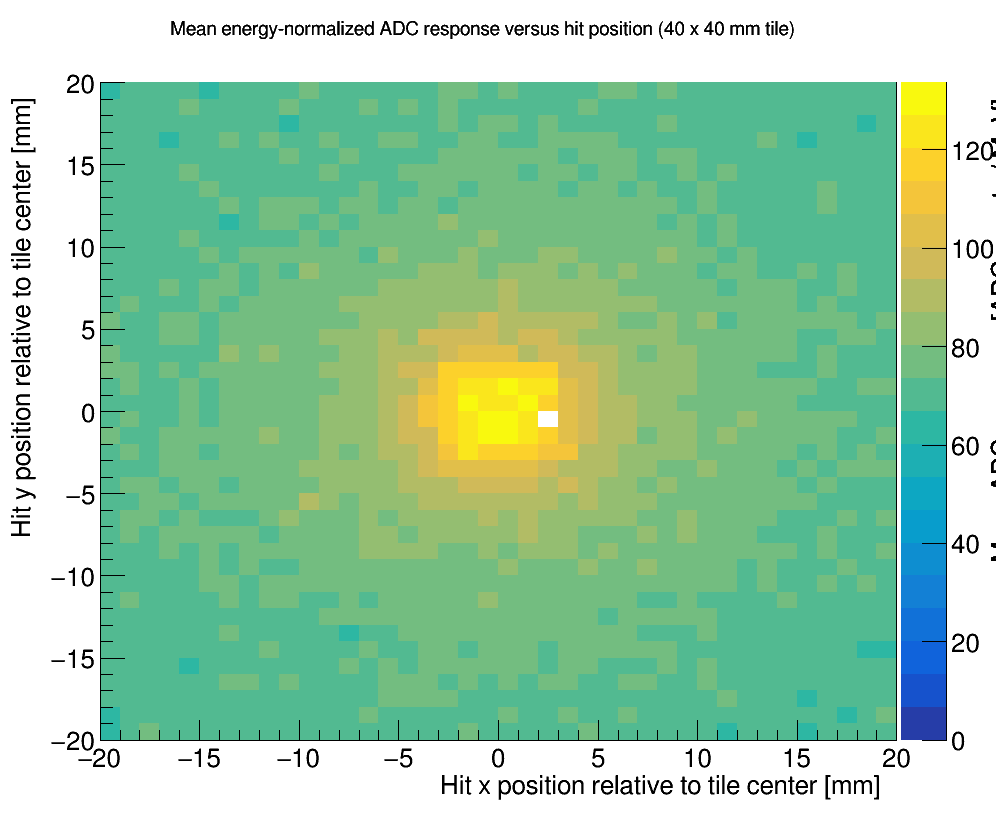
\includegraphics[height=3.0cm]{../analysis/plots/adc/mean_adc_per_mev_vs_position.png}\\[2pt]
      \footnotesize ADC/MeV, energy-normalized
    \end{column}
  \end{columns}
  \vspace{4pt}
  \footnotesize
  Spatial uniformity map of the raw response and energy-normalized map
  for tiles $40\times40~\mathrm{mm^2}$. Empty bins mark regions without
  selected events, not zero response.
\end{frame}

\begin{frame}{Individual Per-Particle Mean-ADC-vs-Energy Curves}
  \begin{columns}[T]
    \begin{column}{0.5\textwidth}
      \centering
      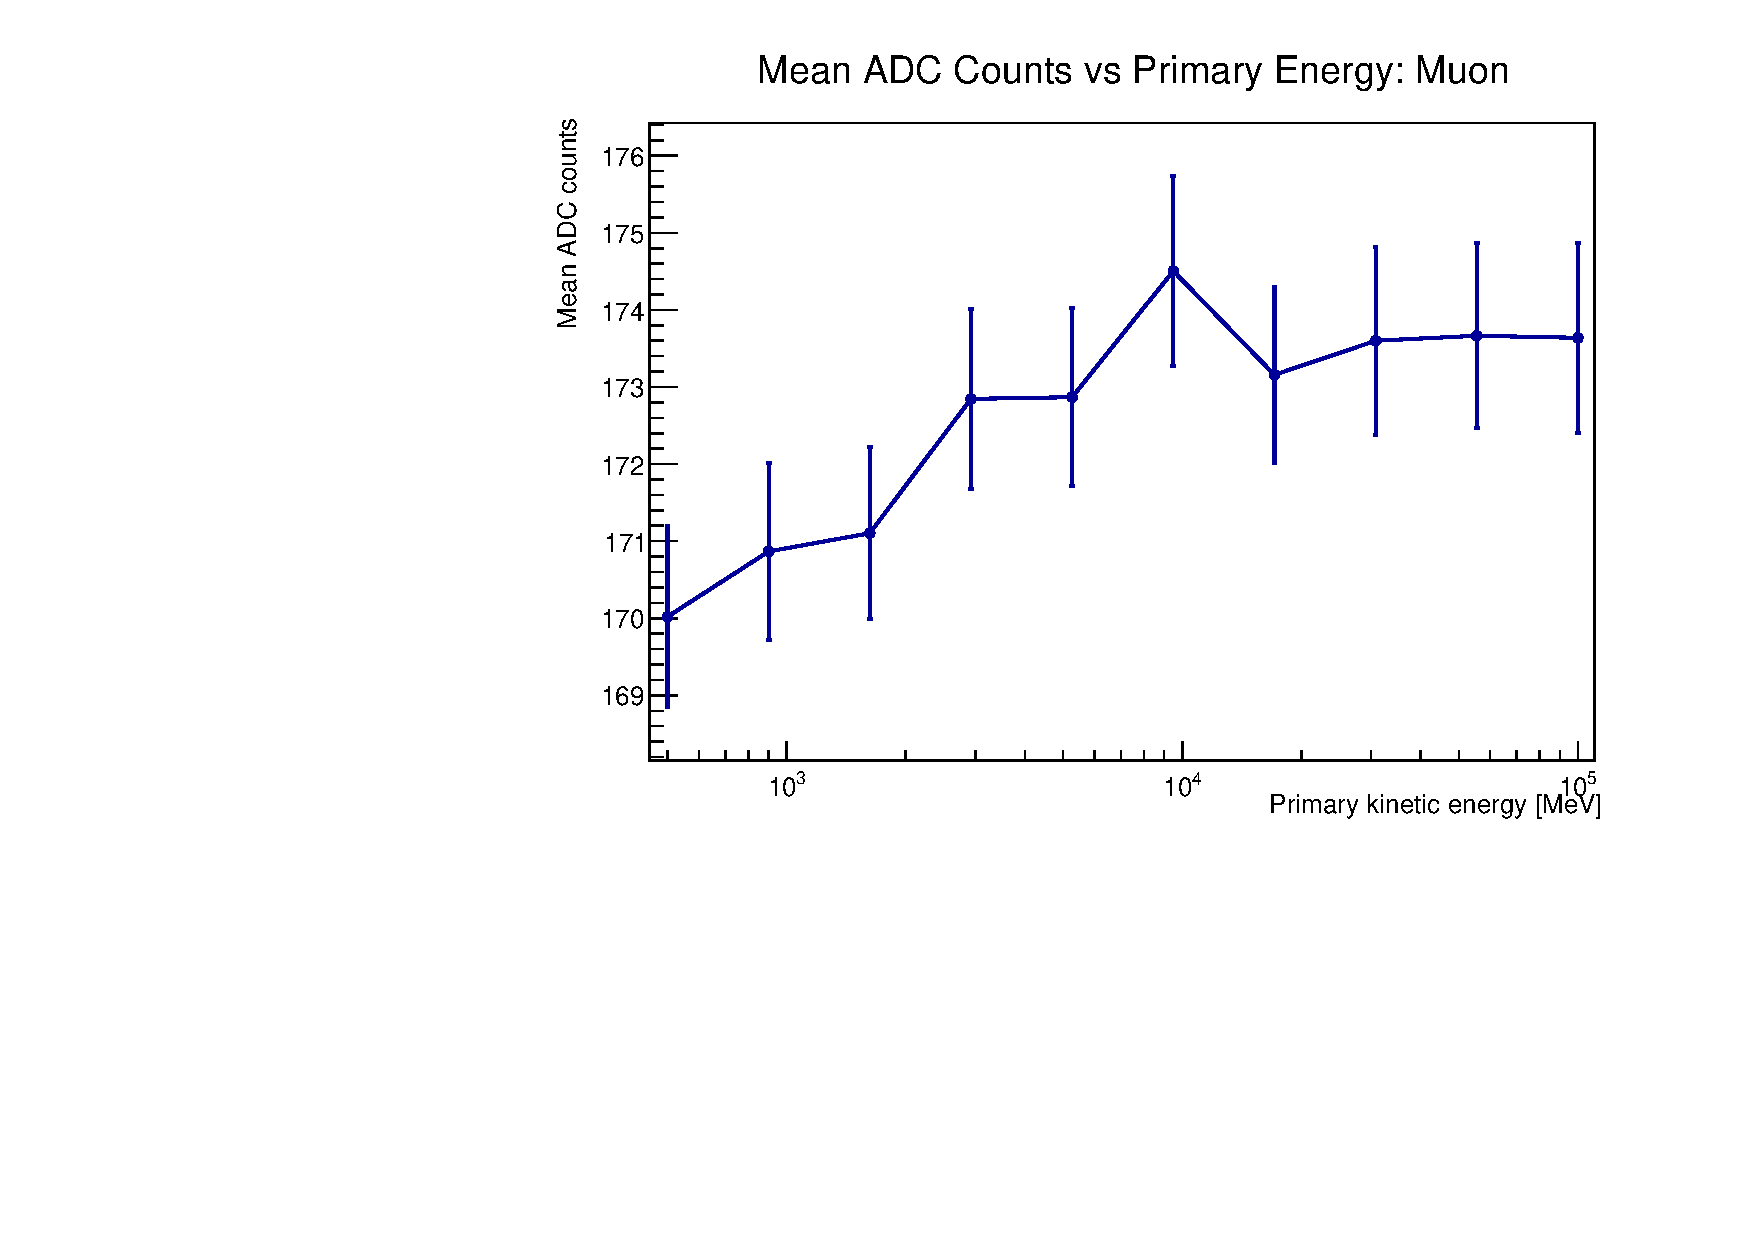
\includegraphics[height=3.0cm]{../analysis/plots/energy_scan/adc_vs_energy_muon.pdf}\\[2pt]
      \footnotesize \muminus: 0.5--100\,GeV
    \end{column}
    \begin{column}{0.5\textwidth}
      \centering
      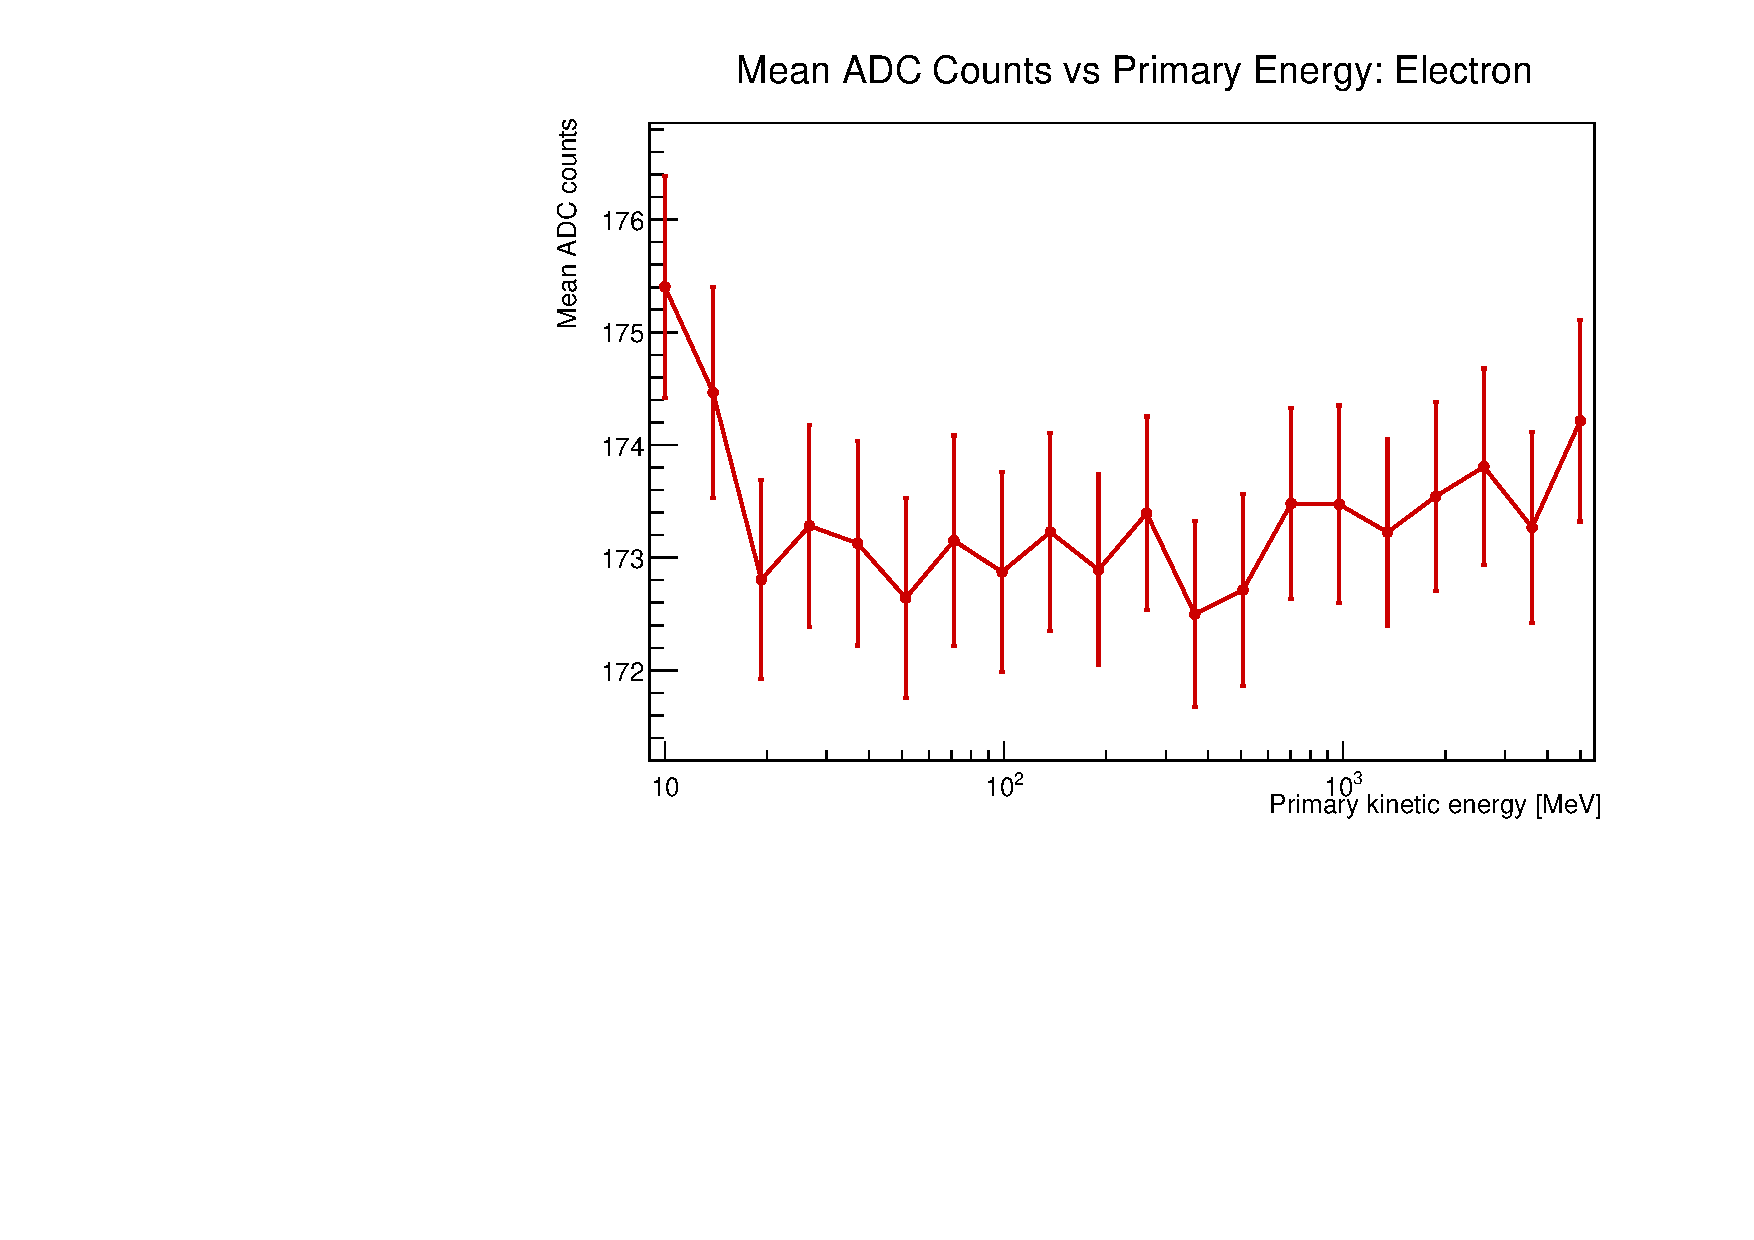
\includegraphics[height=3.0cm]{../analysis/plots/energy_scan/adc_vs_energy_electron.pdf}\\[2pt]
      \footnotesize \eminus: 0.05\,MeV--2\,GeV, 20 points
    \end{column}
  \end{columns}
  \vspace{4pt}
  \footnotesize
  Muon response is essentially flat (mild relativistic rise). The
  electron scan resolves the absorbed-to-punch-through transition:
  trigger onset $\approx 0.27$\,MeV, containment peak $\approx 190$ ADC
  at 4.3\,MeV, settling onto the 172--174-count MIP plateau above
  13\,MeV.
\end{frame}

\begin{frame}{Photon Response, Split by Interaction}
  \begin{columns}[T]
    \begin{column}{0.5\textwidth}
      \centering
      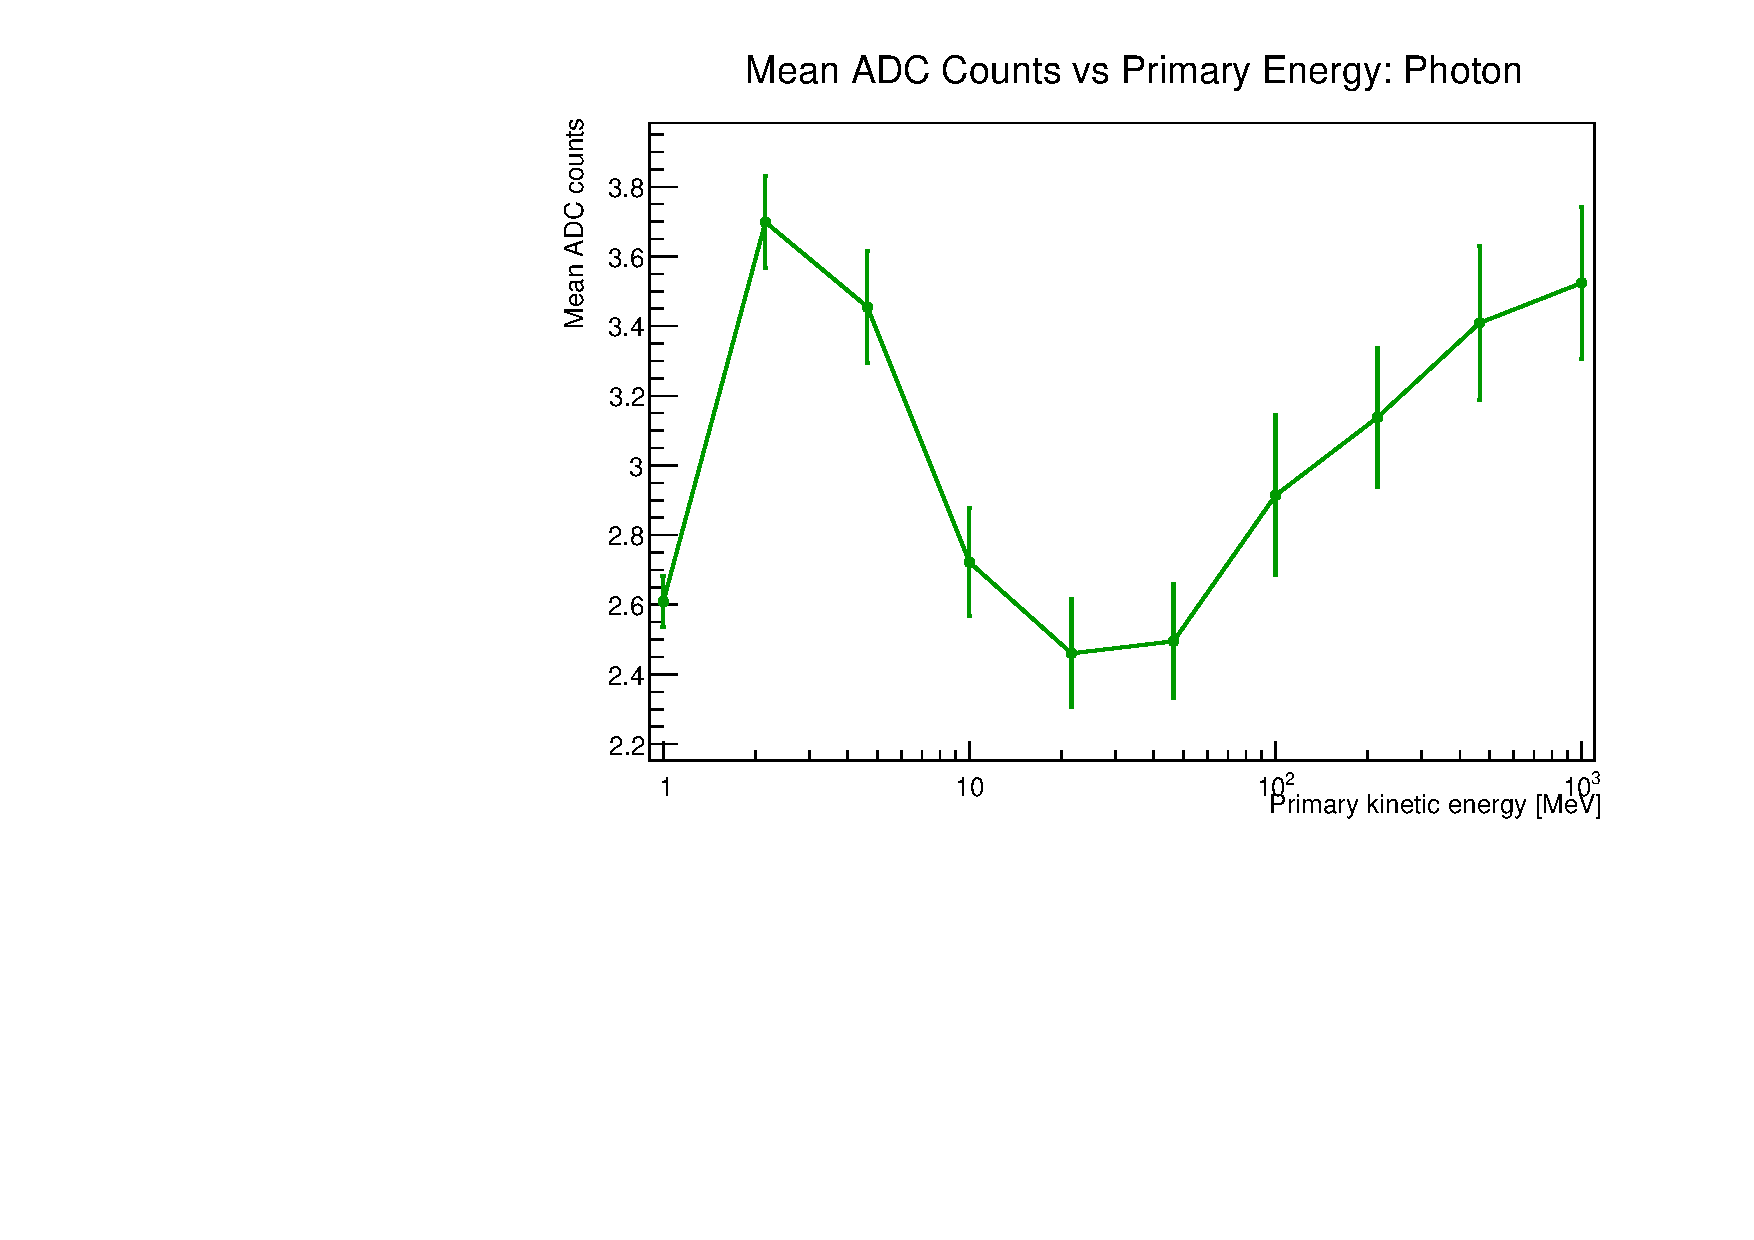
\includegraphics[height=3.0cm]{../analysis/plots/energy_scan/adc_vs_energy_photon_all.pdf}\\[2pt]
      \footnotesize All \gam\ events, interacted or not
    \end{column}
    \begin{column}{0.5\textwidth}
      \centering
      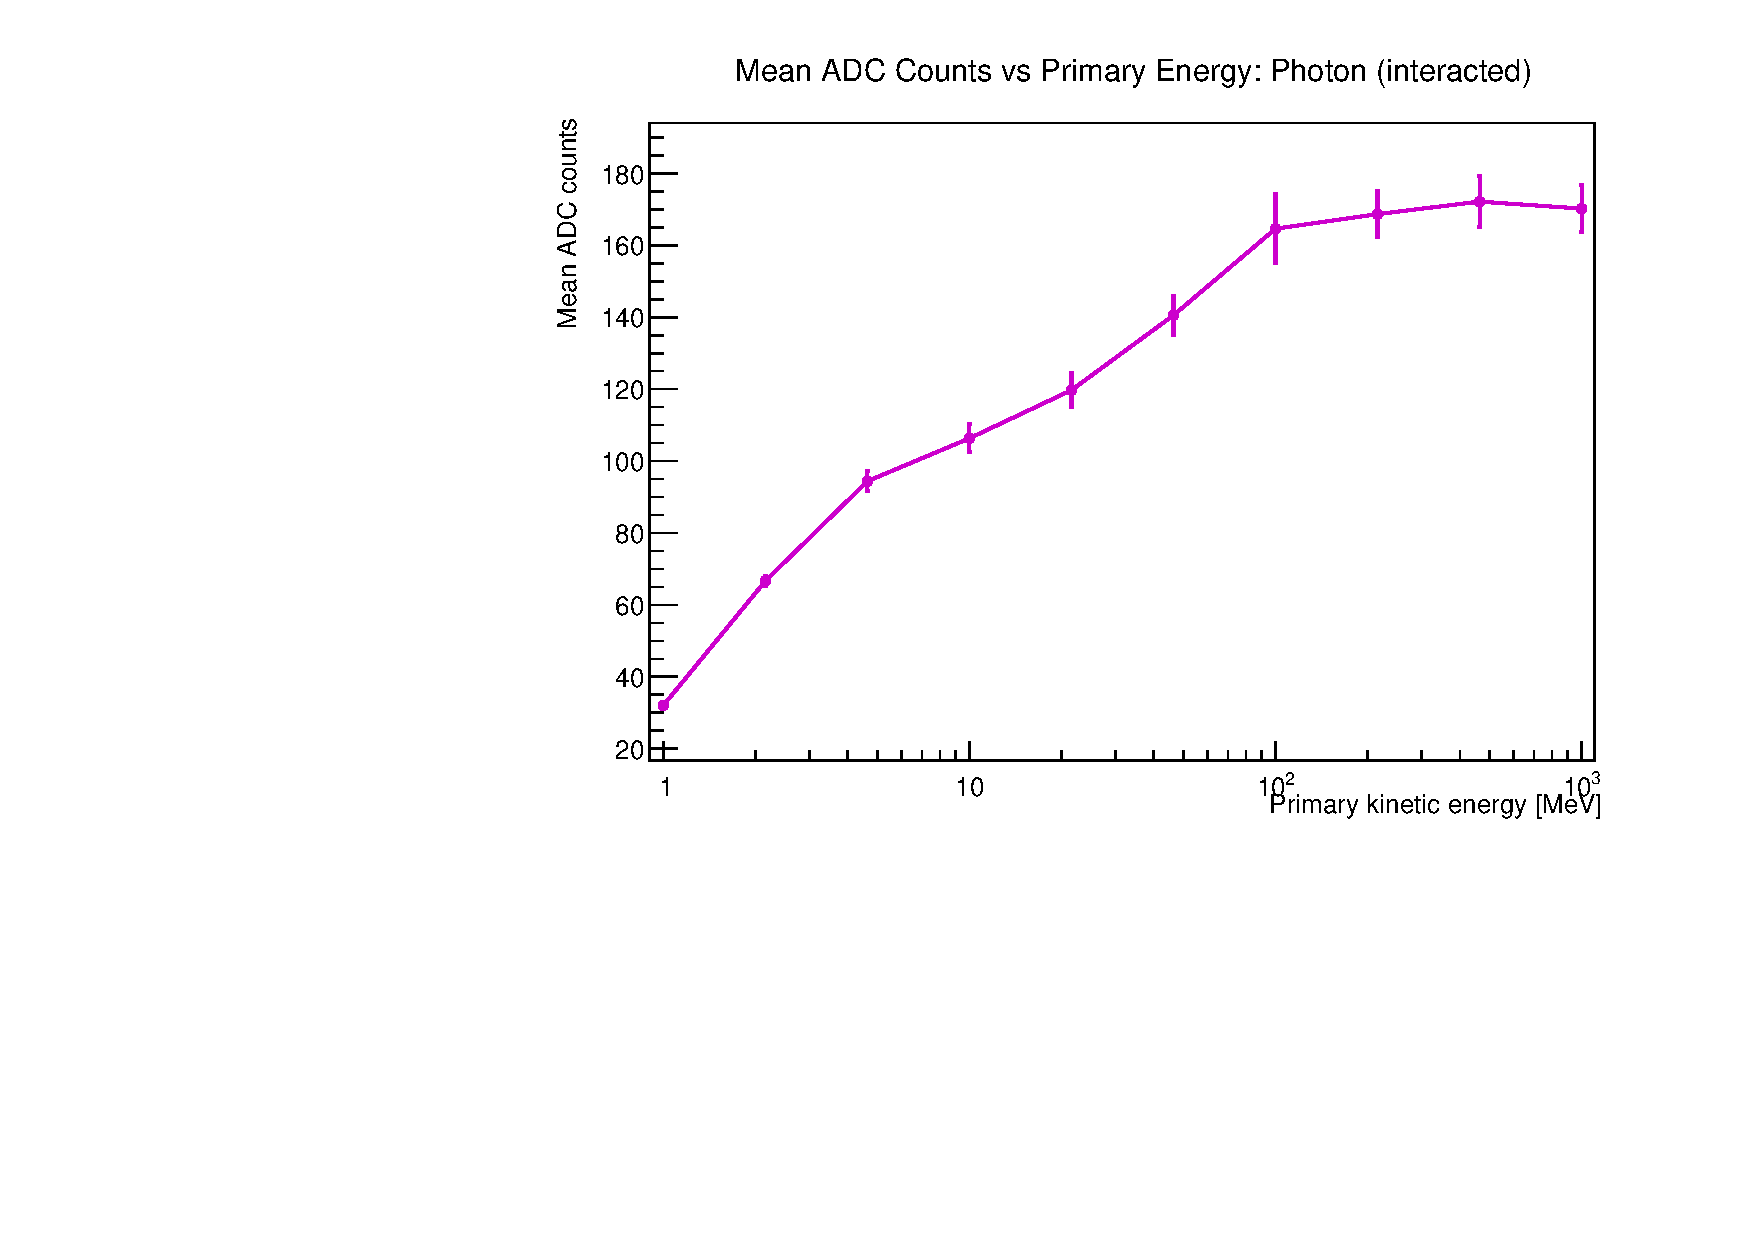
\includegraphics[height=3.0cm]{../analysis/plots/energy_scan/adc_vs_energy_photon_interacted.pdf}\\[2pt]
      \footnotesize Only interacted \gam\ events
    \end{column}
  \end{columns}
  \vspace{4pt}
  \footnotesize
  The all-events curve is dominated by the low interaction probability
  in the thin tile and stays near zero. Restricting to non-zero deposits
  reveals a rise $\to$ peak $\to$ MIP-like plateau comparable to
  \muminus/\eminus\ at high energy.
\end{frame}

\begin{frame}{Two Levels of the Final UBT Mapping}
  \begin{columns}[T]
    \begin{column}{0.5\textwidth}
      \centering
      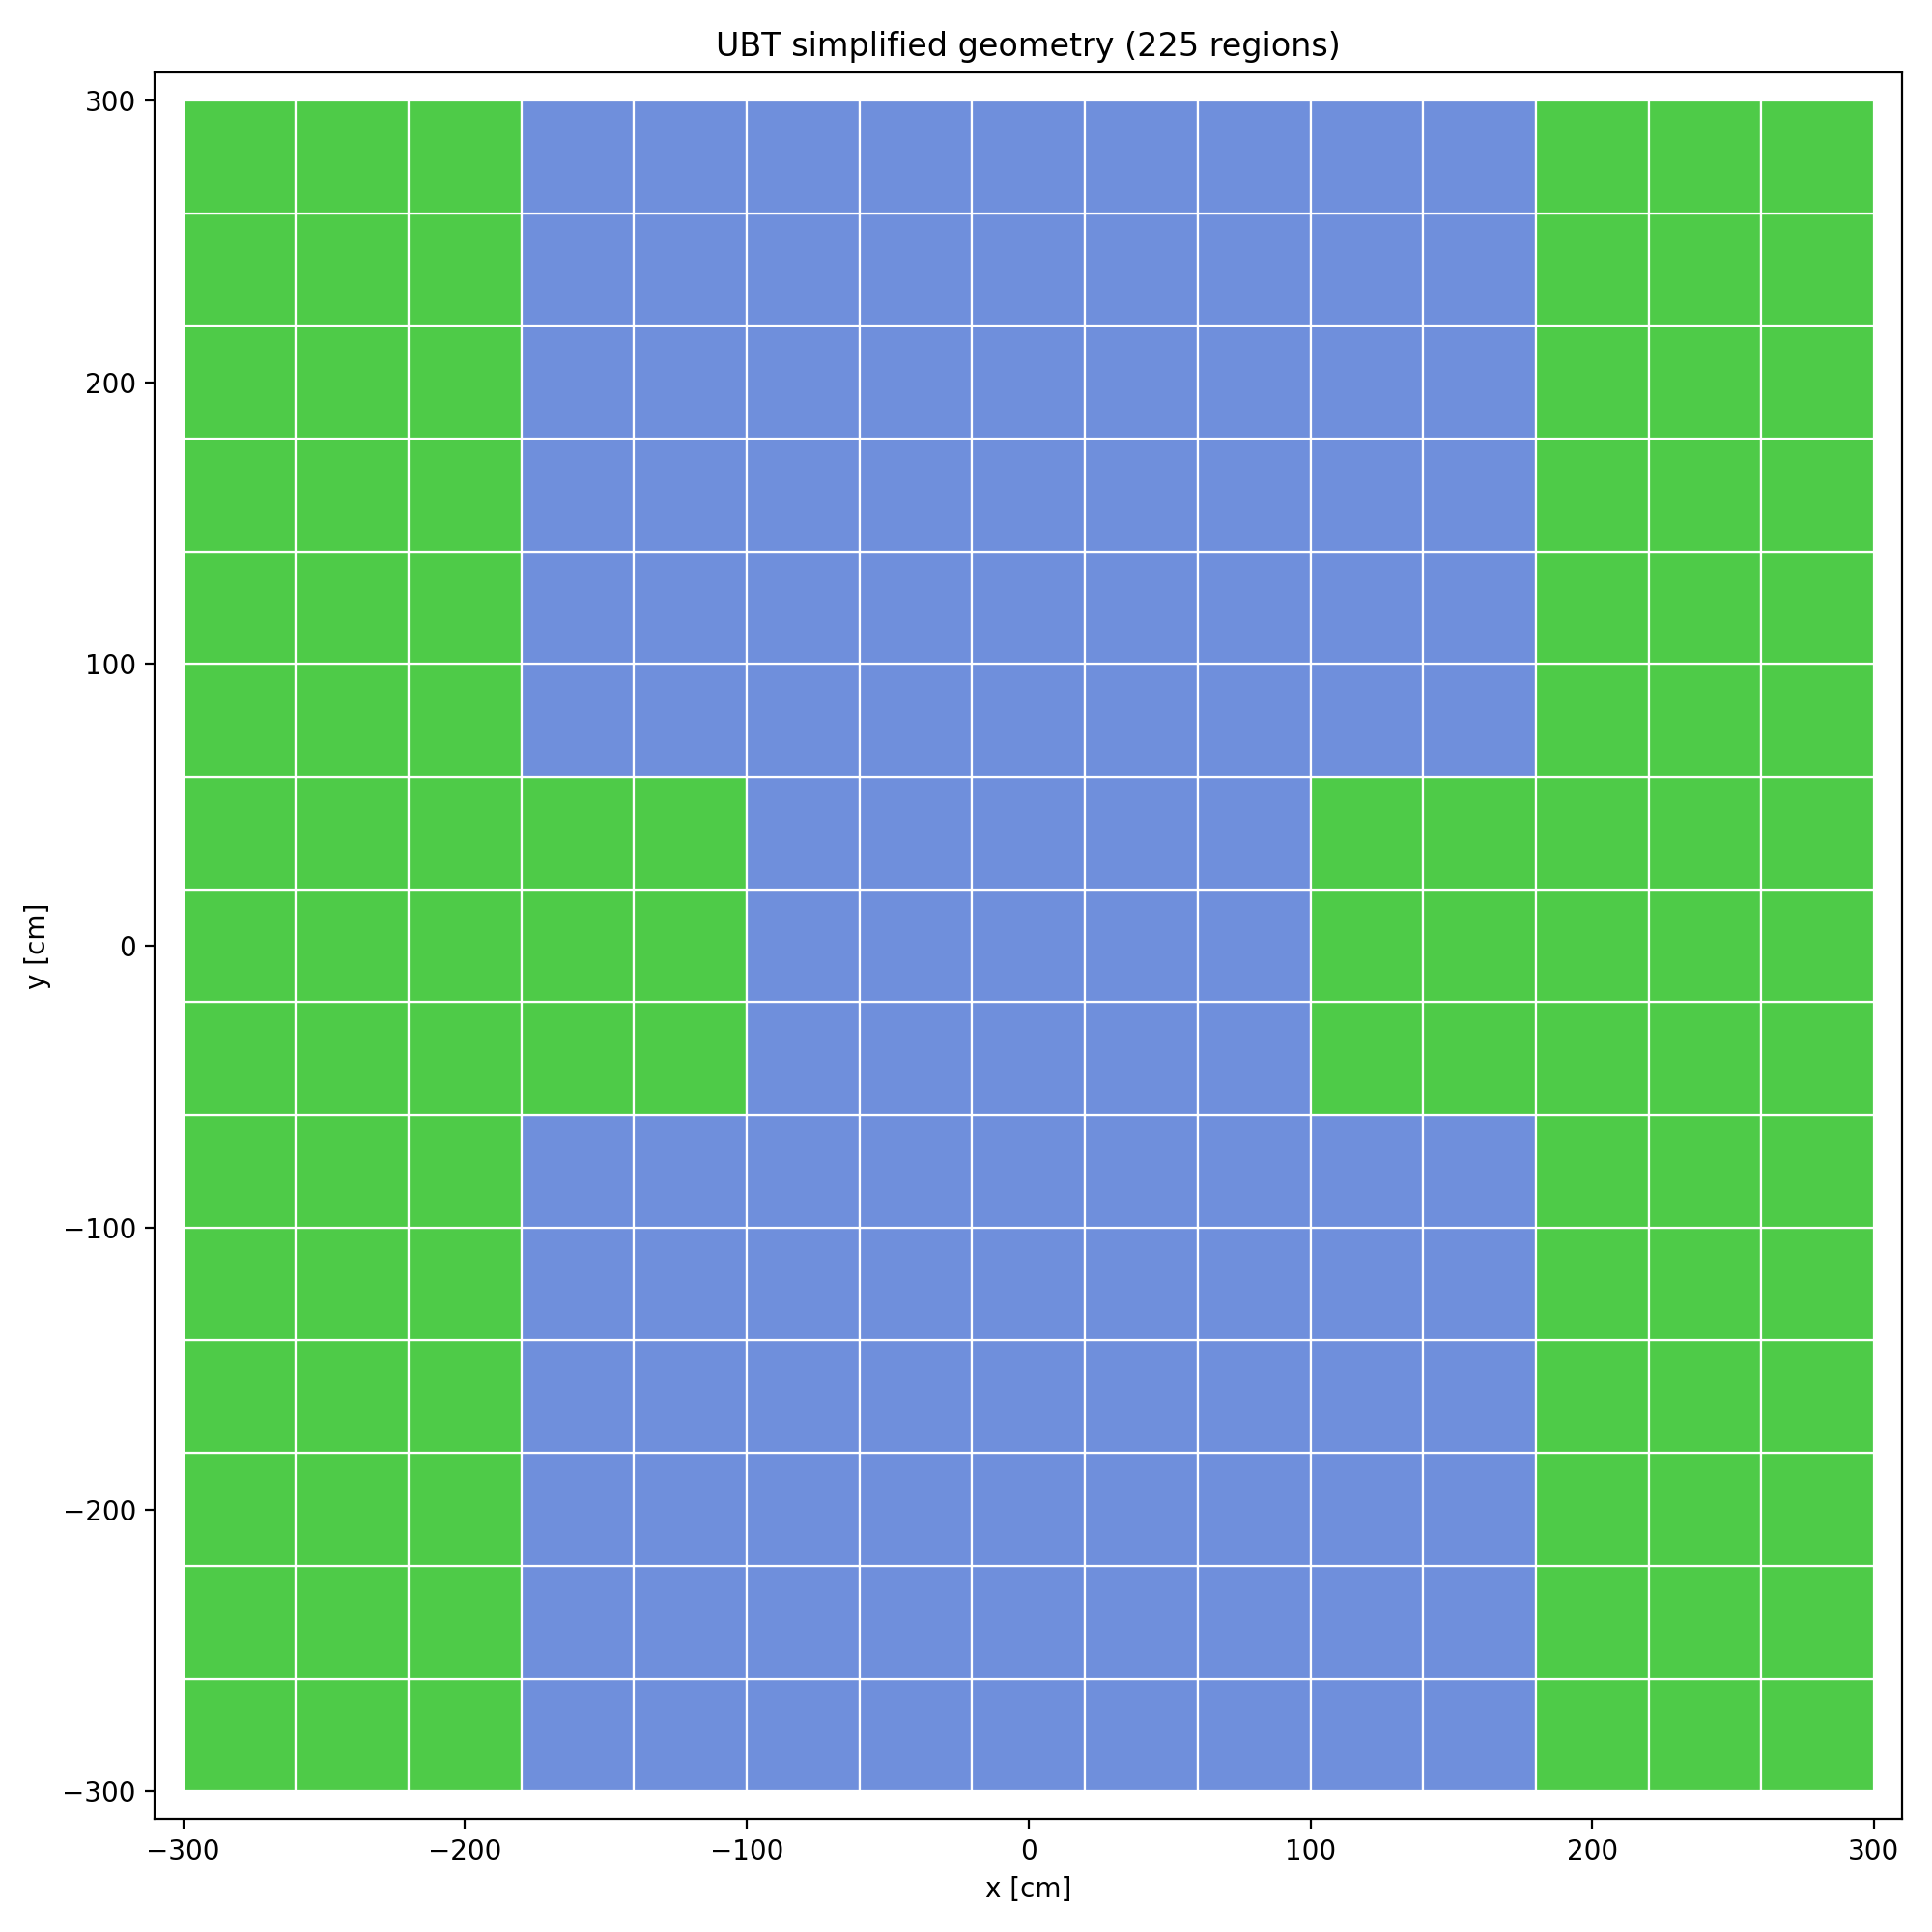
\includegraphics[height=3.3cm]{../geometry/ubt_geometry_simulation.png}\\[2pt]
      \footnotesize Coarse transport map: 225 regions of $40\times40~\mathrm{cm^2}$
    \end{column}
    \begin{column}{0.5\textwidth}
      \centering
      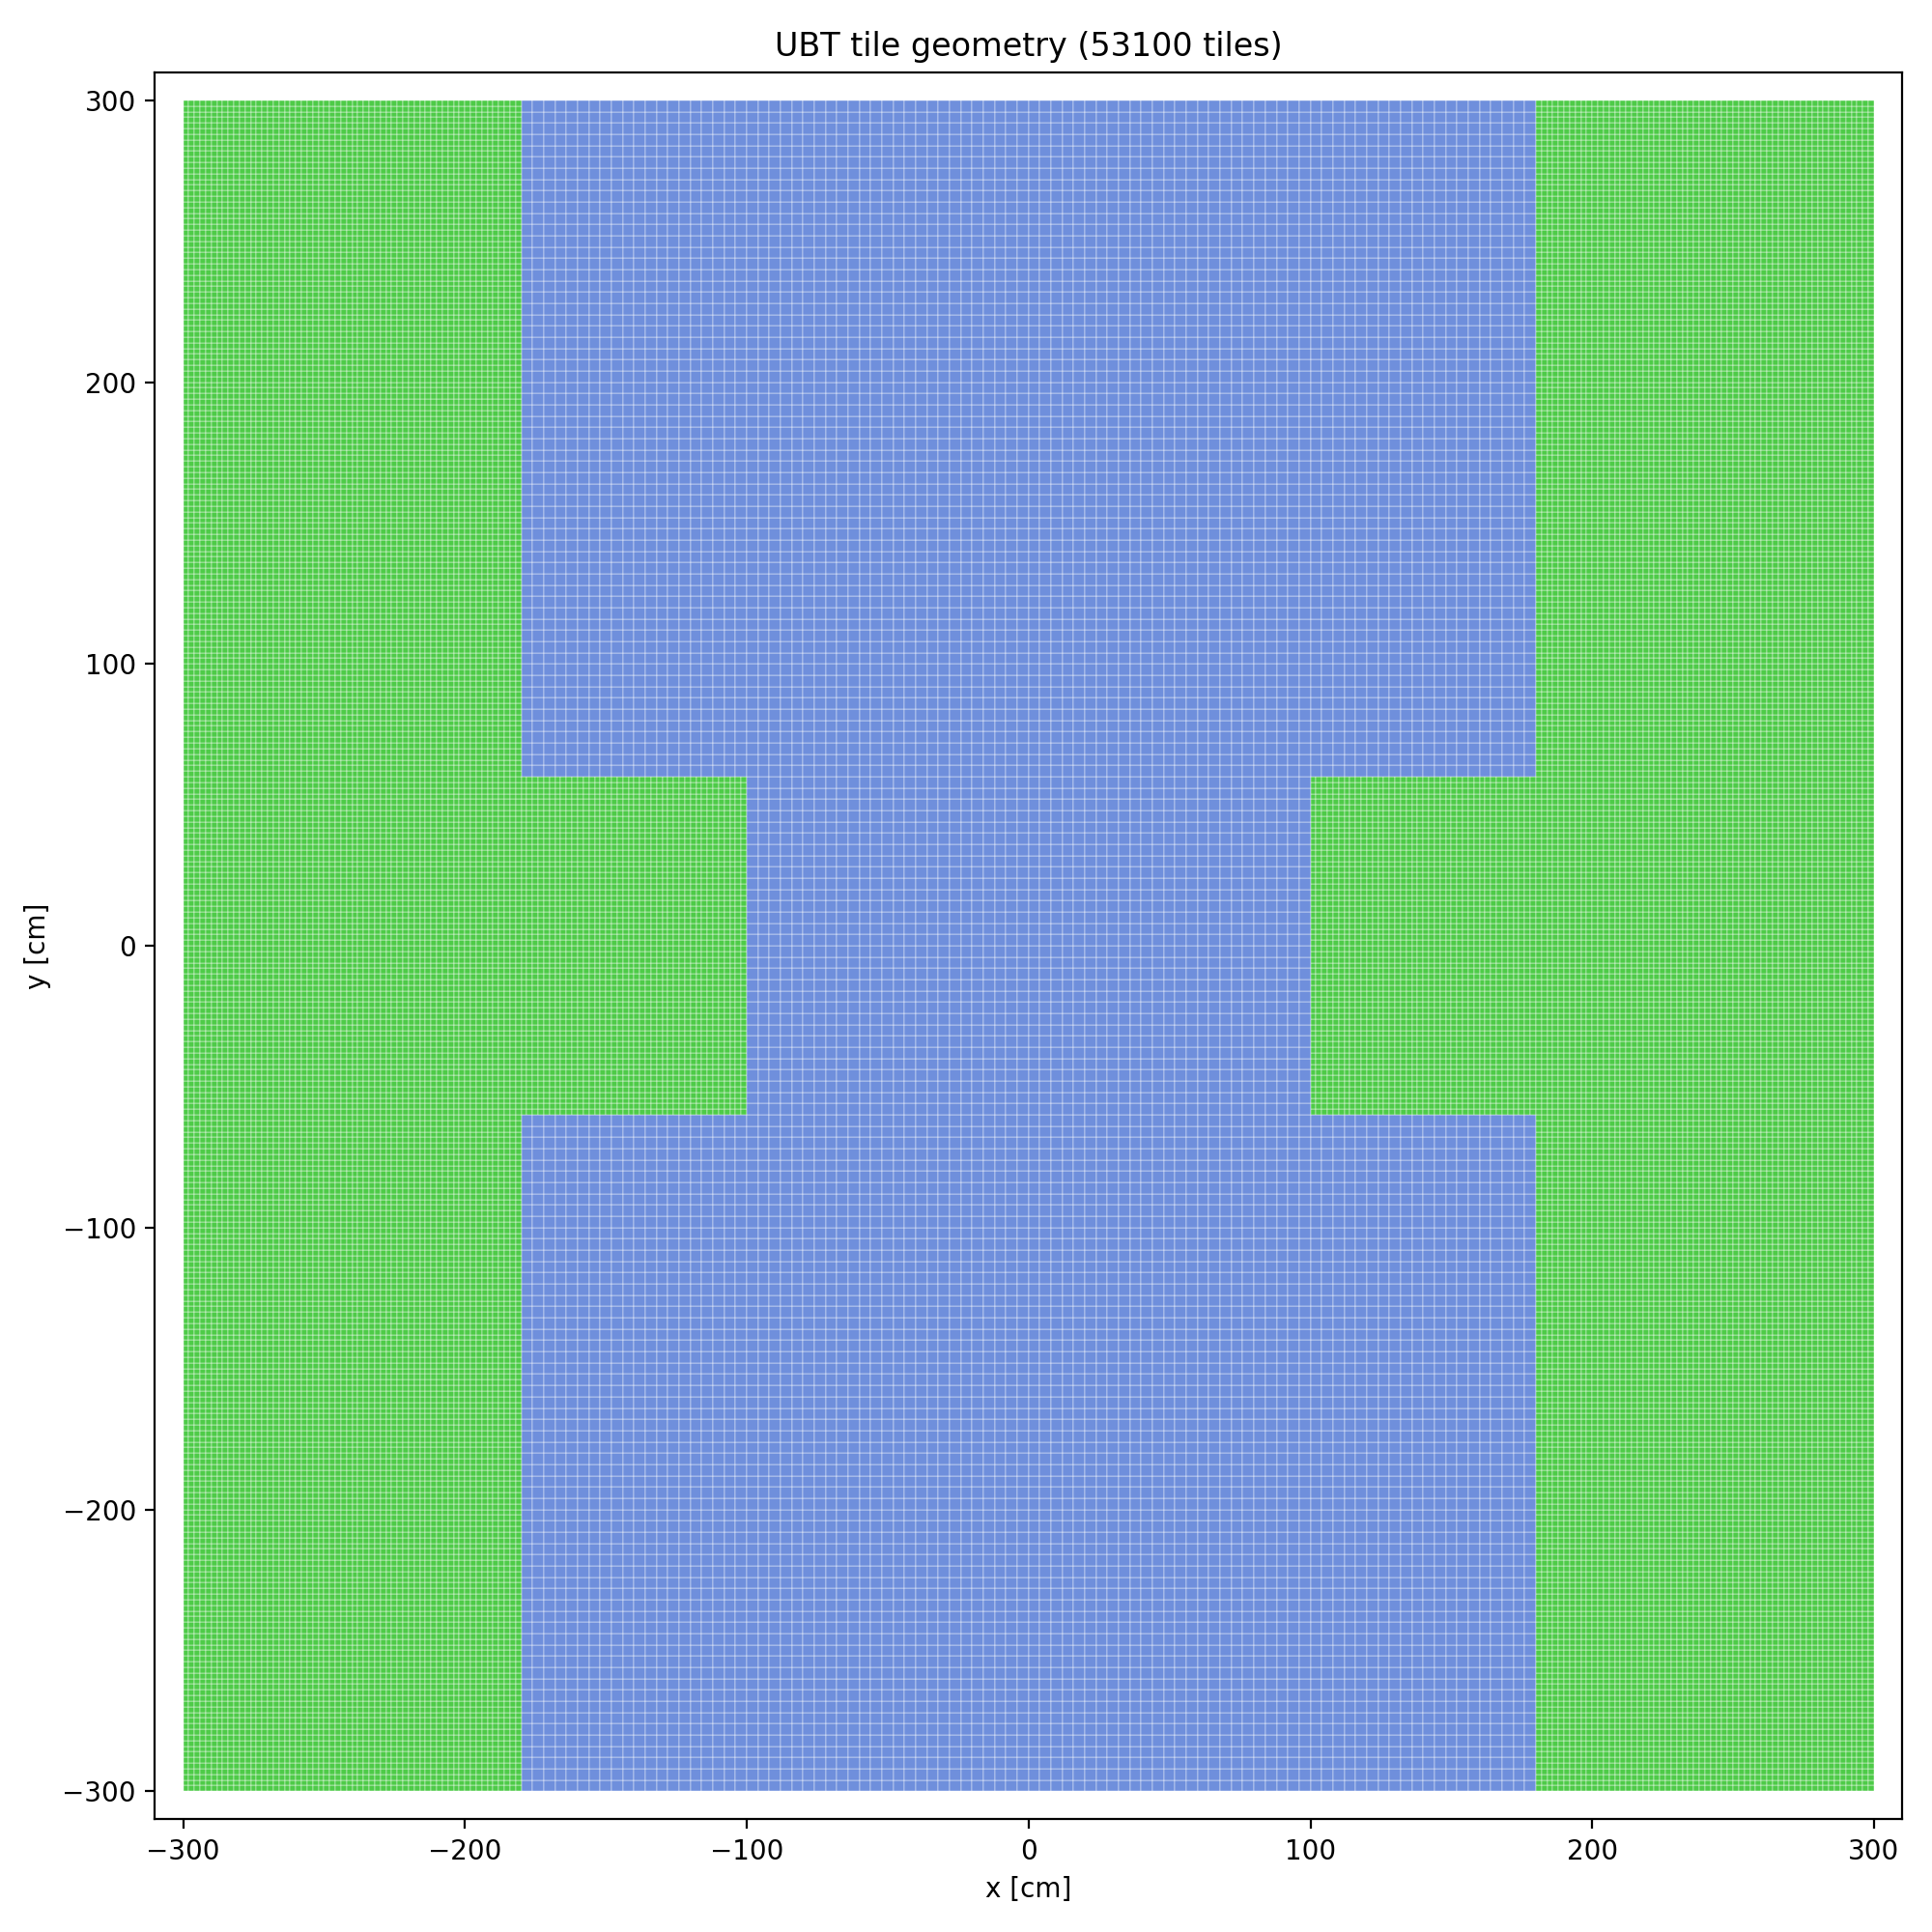
\includegraphics[height=3.3cm]{../geometry/ubt_geometry_digitization.png}\\[2pt]
      \footnotesize Constituent-tile map for digitized hit coordinates
    \end{column}
  \end{columns}
  \vspace{4pt}
  \footnotesize
  Only the coarse regions (left) are physical FairShip geometry volumes;
  the small tiles (right) are inferred mathematically during
  digitization. Blue: $4\times4~\mathrm{cm^2}$ tiles; green:
  $2\times2~\mathrm{cm^2}$ tiles (three-column full-height sides,
  two-column-per-side central neck).
\end{frame}

% ============================================================================
\section{FairShip Digitization \& Expected Rates}
% ============================================================================

\begin{frame}{FairShip Digitization: Coarse Plane to Small-Tile ADC}
  \begin{columns}[T]
    \begin{column}{0.52\textwidth}
      \footnotesize
      \textbf{From physical volumes to a small-tile response, in short:}
      \begin{enumerate}
        \item Transport only sees \alert{coarse} regions: a $15\times15$
          grid of 225 sensitive $40\times40~\mathrm{cm^2}$ volumes, each
          locked to a 2\,cm or 4\,cm constituent-tile pitch (102 vs.\
          123 regions).
        \item Every MC point is \alert{requantized} onto the implicit
          small tile: $i_q=\lfloor (q_\mathrm{MC}-o)/s(D)\rfloor$ picks
          the tile index; the digitized position becomes that
          \emph{small tile's center}, not the parent region's.
        \item ADC uses the point's \alert{exact local position} inside
          the small tile, $x_\mathrm{local}=x_\mathrm{MC}-x_\mathrm{tile}$,
          looked up in a $1\times1~\mathrm{mm^2}$ ADC/MeV map from the
          standalone Geant4 study.
        \item $N_\mathrm{ADC}=\mathrm{round}\!\big(E_\mathrm{dep}[\mathrm{MeV}]
          \cdot R_s(x_\mathrm{local},y_\mathrm{local})\big)$; triggered
          when $N_\mathrm{ADC}\ge100$.
      \end{enumerate}
    \end{column}
    \begin{column}{0.48\textwidth}
      \centering
      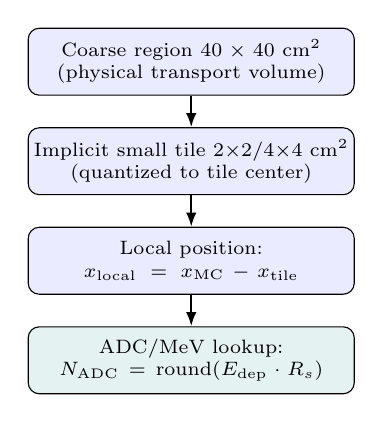
\begin{tikzpicture}[
        node distance=4mm,
        box/.style={draw, rounded corners, fill=blue!8, align=center,
          text width=4.0cm, font=\scriptsize, inner sep=2pt,
          minimum height=0.85cm},
        arr/.style={-{Latex[length=1.8mm]}, thick}
      ]
        \node[box] (a) {Coarse region $40\times40~\mathrm{cm^2}$\\(physical transport volume)};
        \node[box, below=of a] (b) {Implicit small tile $2\!\times\!2$/$4\!\times\!4~\mathrm{cm^2}$\\(quantized to tile center)};
        \node[box, below=of b] (c) {Local position: $x_\mathrm{local}=x_\mathrm{MC}-x_\mathrm{tile}$};
        \node[box, below=of c, fill=teal!10] (d) {ADC/MeV lookup:\\$N_\mathrm{ADC}=\mathrm{round}(E_\mathrm{dep}\cdot R_s)$};
        \draw[arr] (a) -- (b);
        \draw[arr] (b) -- (c);
        \draw[arr] (c) -- (d);
      \end{tikzpicture}
    \end{column}
  \end{columns}
\end{frame}

\begin{frame}{Expected Particle Rate per Tile}
  \begin{columns}[T]
    \begin{column}{0.5\textwidth}
      \centering
      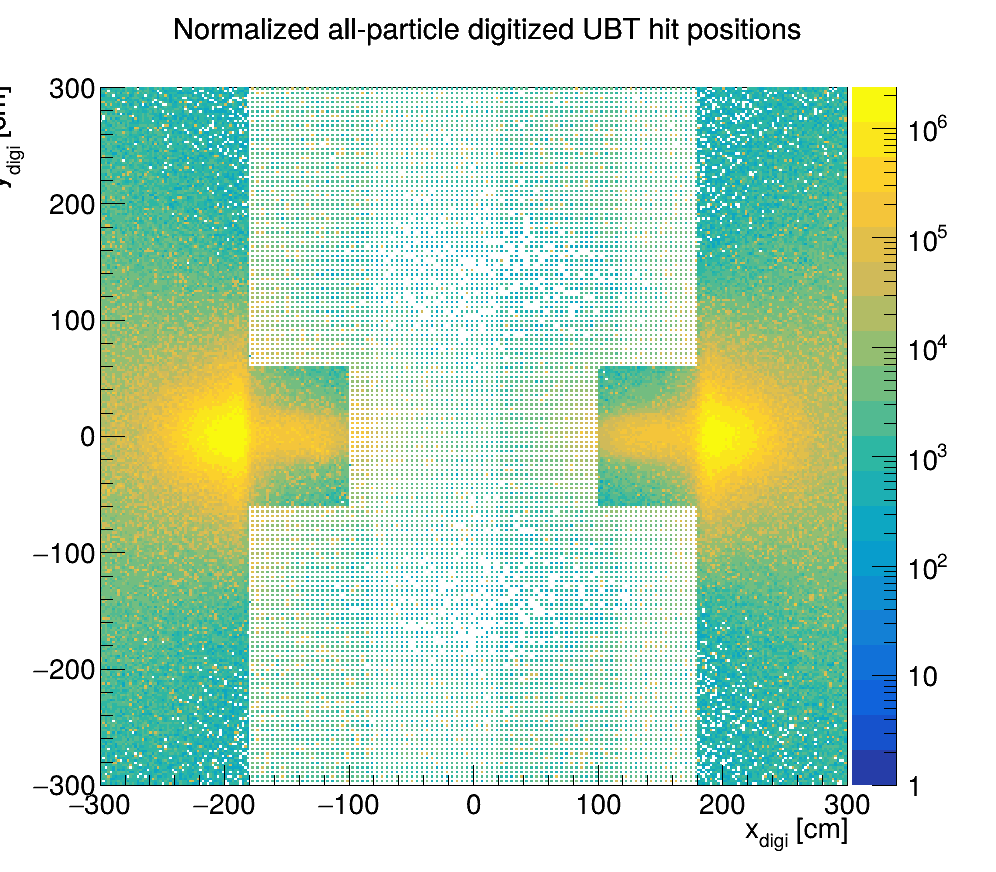
\includegraphics[height=2.9cm]{figs/ubt_digitized_hits.png}\\[2pt]
      \footnotesize General spatial rate map, all species (weighted, log $z$)
    \end{column}
    \begin{column}{0.5\textwidth}
      \centering
      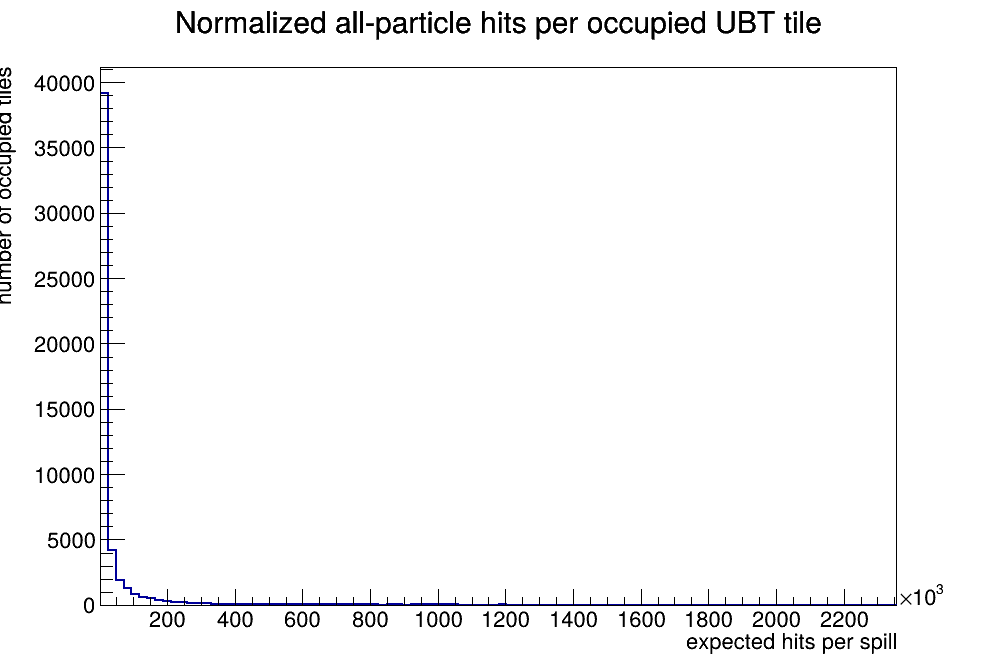
\includegraphics[height=2.9cm]{figs/ubt_digitized_hits_hits_per_tile.png}\\[2pt]
      \footnotesize Per-tile expected hit-rate distribution
    \end{column}
  \end{columns}
  \vspace{4pt}
  \footnotesize
  Digitized \texttt{UpstreamTaggerHit} rates over the full detector plane
  from the MinBias2026 muon-background sample, weighted to
  $N_\mathrm{total}=4.12\times10^{8}$ muon-background events per spill
  (\texttt{FairShipUBT/analyze\_ubt\_hits.py}). Under the standard
  $\approx 1$\,s SHiP spill convention, hits/spill are read as an
  approximate rate in Hz; the rate peaks near the beam axis, where a few
  tiles exceed 1\,MHz.
\end{frame}

\begin{frame}{Expected Rate per Particle Type}
  \begin{columns}[T]
    \begin{column}{0.333\textwidth}
      \centering
      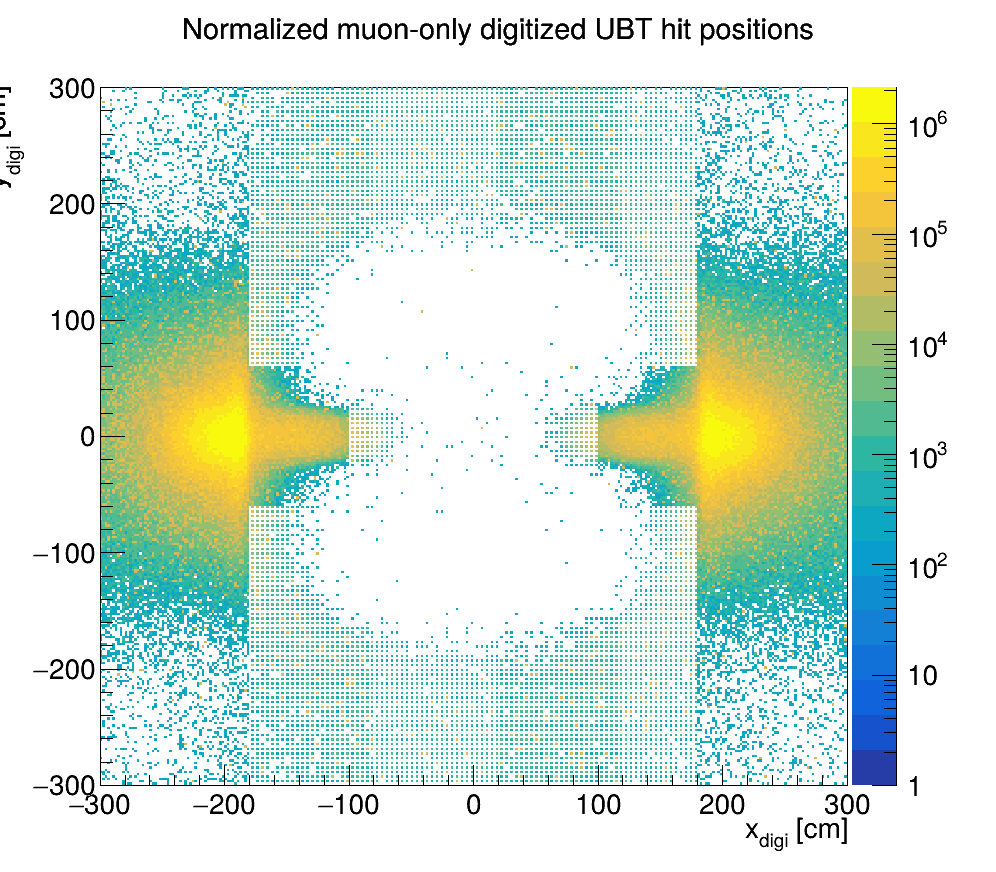
\includegraphics[height=2.6cm]{figs/ubt_digitized_hits_muon.png}\\[2pt]
      \footnotesize \muminus\ only
    \end{column}
    \begin{column}{0.333\textwidth}
      \centering
      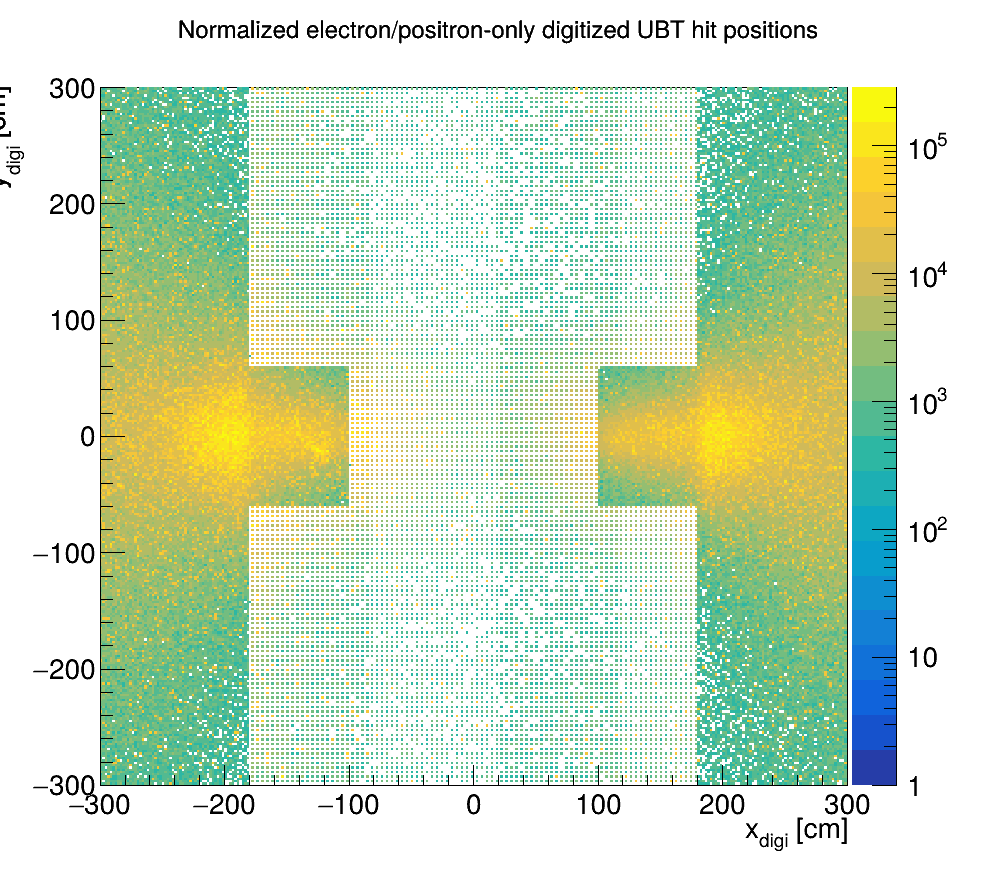
\includegraphics[height=2.6cm]{figs/ubt_digitized_hits_electron.png}\\[2pt]
      \footnotesize \eminus/$e^+$ only
    \end{column}
    \begin{column}{0.333\textwidth}
      \centering
      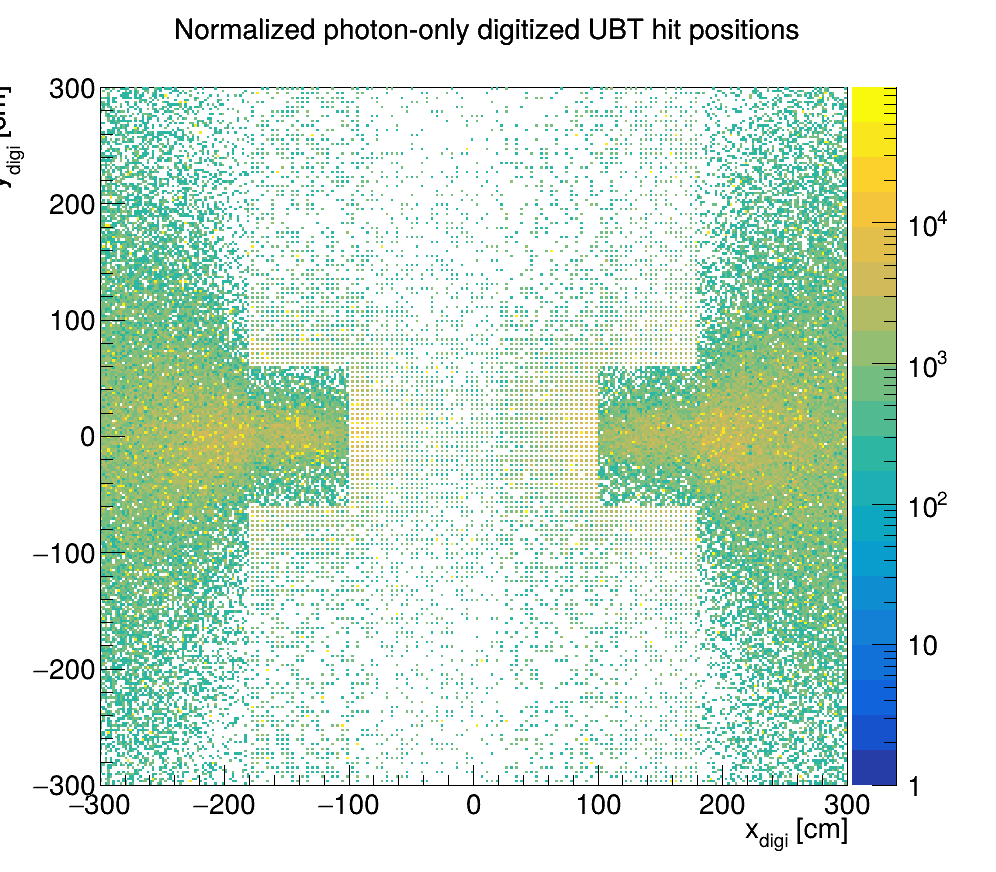
\includegraphics[height=2.6cm]{figs/ubt_digitized_hits_gamma.png}\\[2pt]
      \footnotesize \gam\ only
    \end{column}
  \end{columns}
  \vspace{4pt}
  \footnotesize
  Same weighted spatial rate map as the previous slide, split by MC
  primary species. Muons dominate the rate across the whole plane;
  electrons/positrons and photons are comparatively more concentrated
  close to the beam axis, consistent with their softer momentum spectra.
\end{frame}

\begin{frame}{Momentum Distribution of Each Particle}
  \centering
  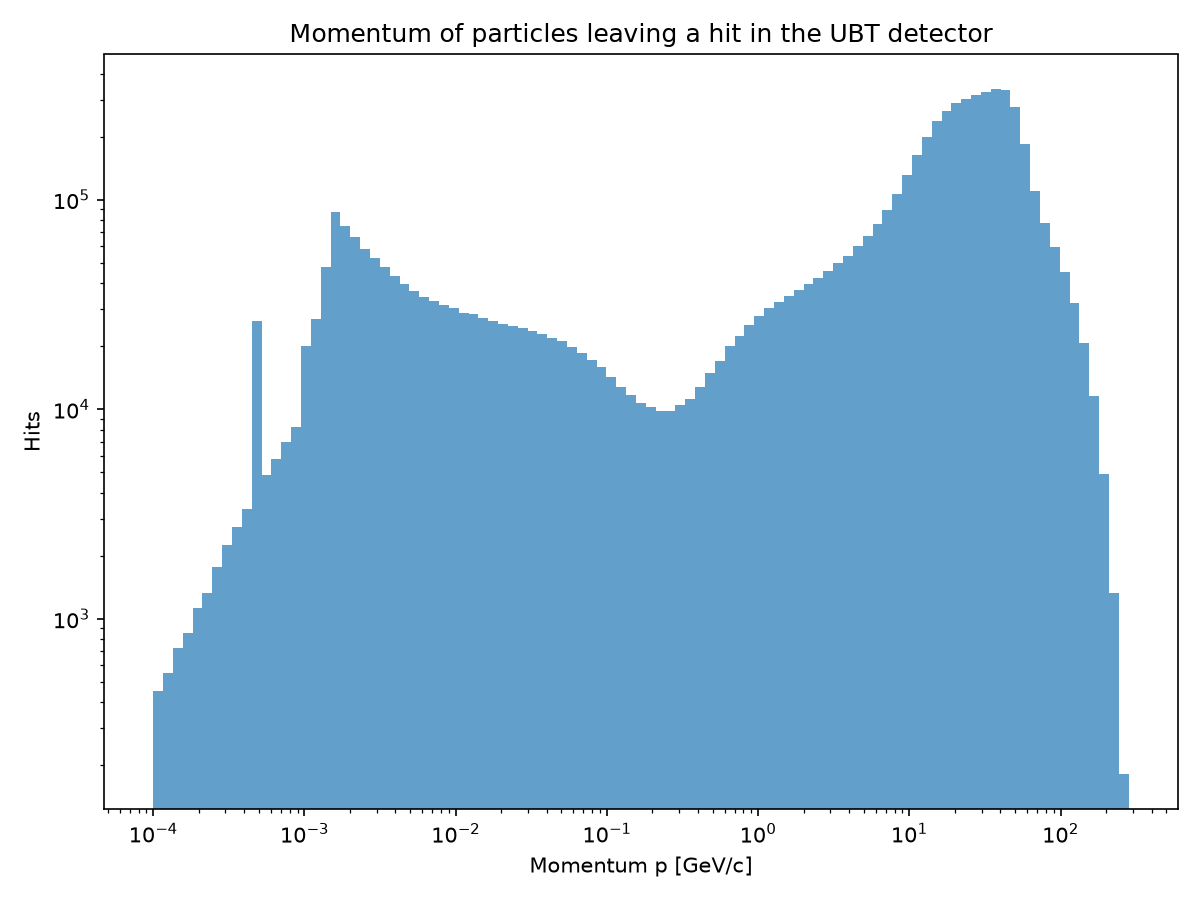
\includegraphics[height=1.9cm]{../analysis/plots/energy_scan/ubt_hit_momentum_all.png}\\[2pt]
  \footnotesize All species combined
  \vspace{3pt}

  \begin{columns}[T]
    \begin{column}{0.333\textwidth}
      \centering
      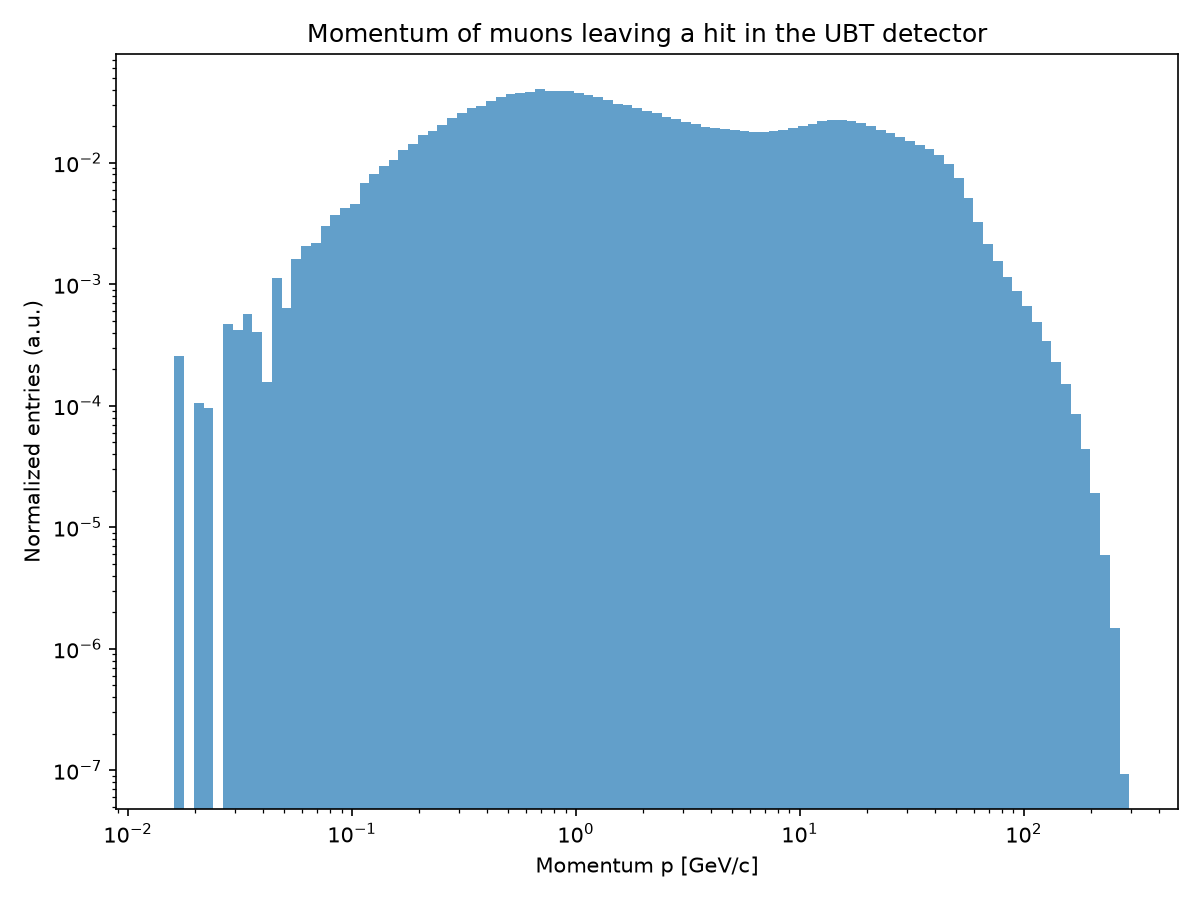
\includegraphics[height=1.9cm]{../analysis/plots/energy_scan/ubt_hit_momentum_muon.png}\\[1pt]
      \tiny \muminus: up to a few hundred GeV$/c$
    \end{column}
    \begin{column}{0.333\textwidth}
      \centering
      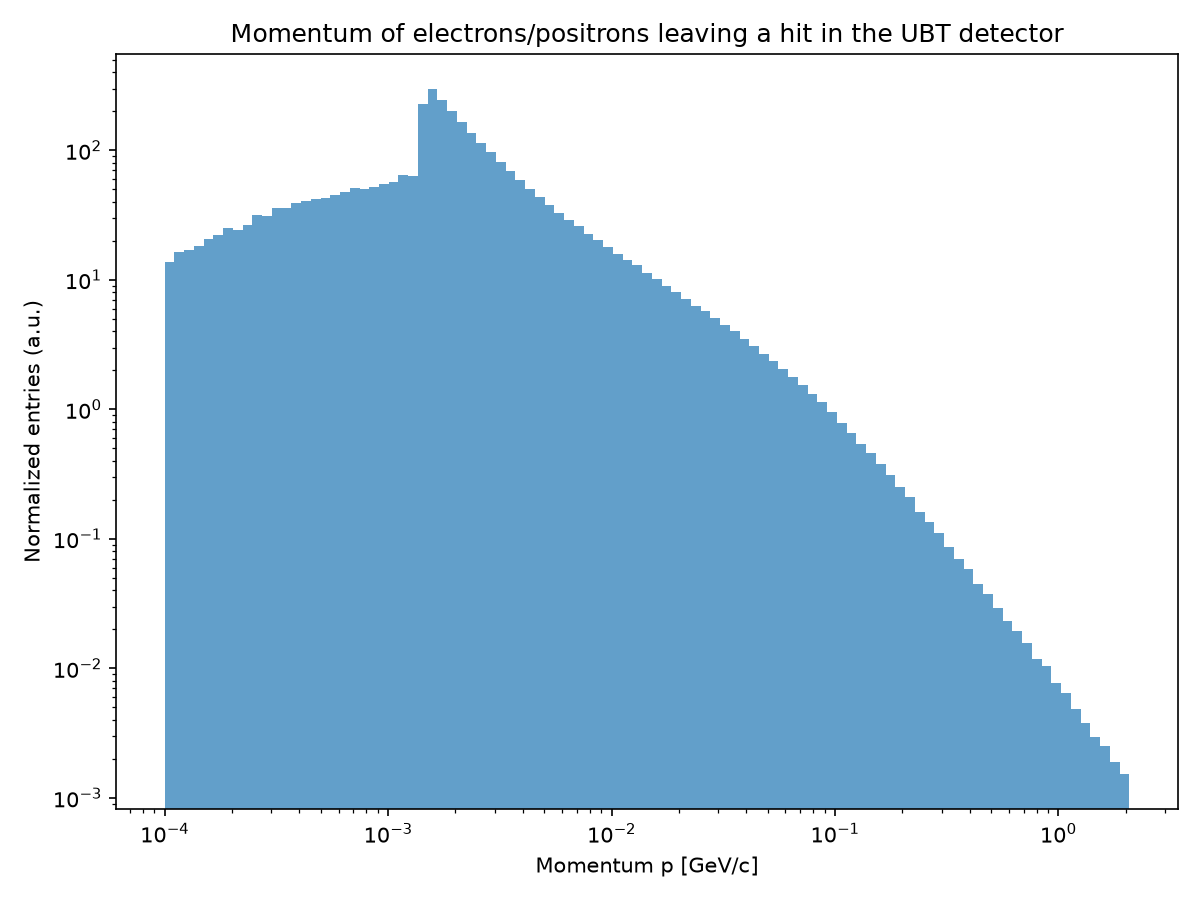
\includegraphics[height=1.9cm]{../analysis/plots/energy_scan/ubt_hit_momentum_electron.png}\\[1pt]
      \tiny \eminus: $\mathcal{O}(1)$\,GeV$/c$
    \end{column}
    \begin{column}{0.333\textwidth}
      \centering
      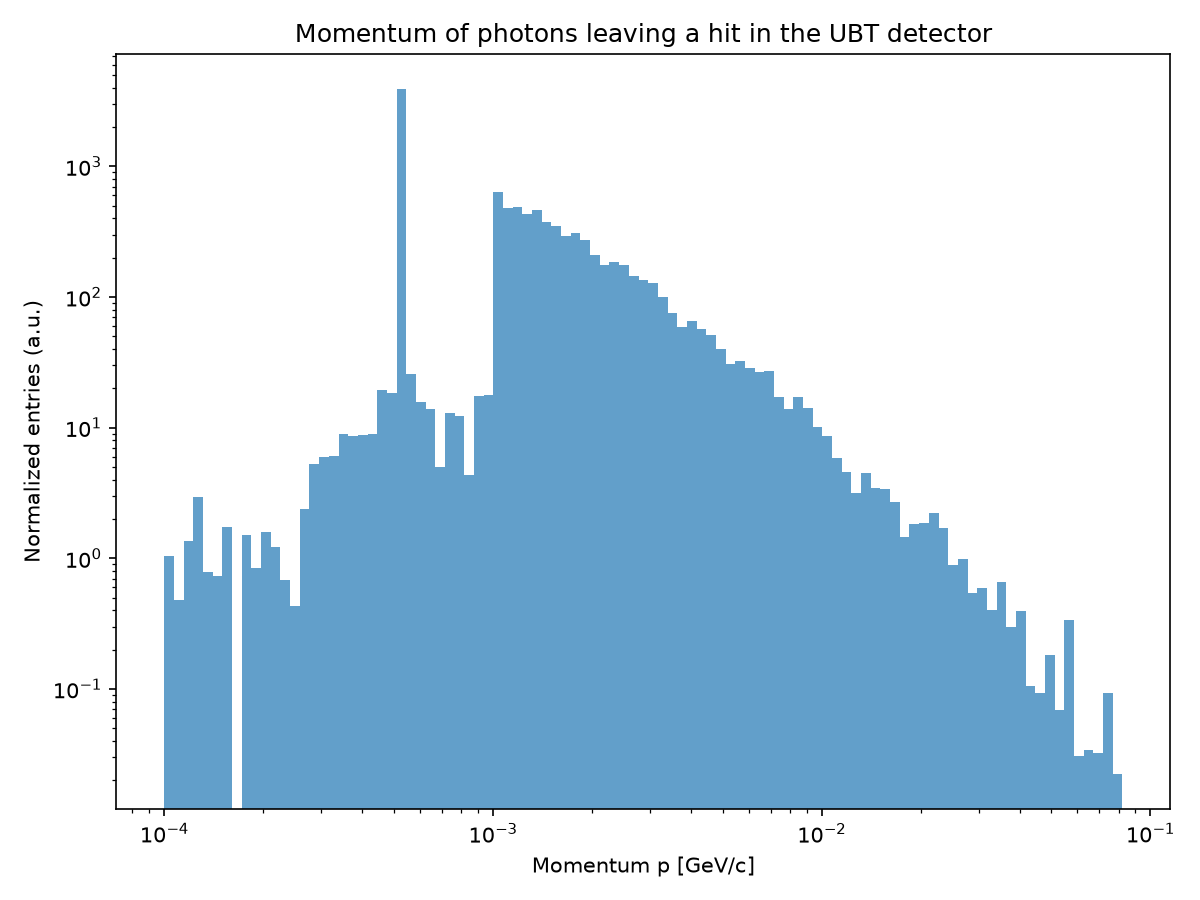
\includegraphics[height=1.9cm]{../analysis/plots/energy_scan/ubt_hit_momentum_gamma.png}\\[1pt]
      \tiny \gam: $\mathcal{O}(10)$\,MeV$/c$
    \end{column}
  \end{columns}
  \vspace{3pt}
  \footnotesize
  Momentum of particles leaving an \texttt{UpstreamTaggerPoint} MC hit
  (same 88-file, 4.13M-event, 5.92M-hit MinBias2026 sample; log-log
  axes). This steeply-falling real spectrum is what the per-particle ADC
  calibration curves are weighted by.
\end{frame}

\end{document}
